\documentclass[10pt, notitlepage]{report}
%\usepackage[utf8]{inputenc}
\usepackage{titlesec}
\usepackage{breakurl}
\usepackage[hyphens]{url}
\usepackage{verbatim}
\usepackage{longtable}
\usepackage{graphicx}
\usepackage{subcaption}
\usepackage{breakcites}
\usepackage{titling}
\usepackage{makecell}

\renewcommand\cellalign{tl}
\renewcommand\cellgape{\Gape[1pt][0pt]}


\usepackage{listings}
\lstset{
  basicstyle=\ttfamily,
  columns=fullflexible,
  frame=single,
  breaklines=true,
  %postbreak=\mbox{\textcolor{red}{$\hookrightarrow$}\space},
}
%Sets the margins 
\usepackage[margin=2.5cm]{geometry}

%Sets the assets path
\graphicspath{{assets/}}

%Removes 'Chapter x' at the start of each section
\titleformat{\chapter}[display] {\normalfont\bfseries}{}{0pt}{\Large}
\titlespacing*{\chapter}{0pt}{-25pt}{30pt}
%Decreases space after subsubsections
\titlespacing{\subsubsection}{0pt}{0\baselineskip}{0\baselineskip}
\titlespacing{\section}{0pt}{10pt}{5pt}


\title{\leavevmode \\\leavevmode \\SpotiMy\\\leavevmode \\}
\author{
	Sandra-Maria Comradi
	\and
	Joseph Cryer
	\and
	Sam Davidson
	\and
	Teodora Dinca
	\and
	Eddy Dunton
	\and
	Fraser Dwyer
	\and
	Sam Freeman
	\and
	Lance Garcia
	\and
	Adam George\\\leavevmode \\
}	
%\date{\leavevmode\\Semester 2,  2019-2020}

\begin{document}

\pagebreak
\hspace{0pt}
\vfill

\thispagestyle{empty}
\section*{\centering CM10251}
\section*{\centering SpotiMy}
\section*{\centering Group 5}
\section*{\centering Semester 2,  2019-2020}

\leavevmode \\
\leavevmode \\
\begin{table}[h]
\centering
\begin{tabular}{p{4cm} p{3cm} p{8cm}}
\textbf{Group Member}&\textbf{Username}&\textbf{Degree Course}\\
\hline
S. Corradi&smc202&MComp Computer Science and Maths, Year 1\\
J. Cryer&jjc82&BSc Computer Science, Year 1\\
S. Davidson&sd2122&BSc Computer Science, Year 1\\
T. Dinca&td598&BSc Computer Science, Year 1\\
E. Dunton&eed34&MComp Computer Science, Year 1\\
F. Dwyer&fd383&BSc Computer Science, Year 1\\
S. Freeman&sf789&MComp Computer Science, Year 1\\
L. Garcia&lg826&BSc Computer Science, Year 1\\
A. George&ad2479&MComp Computer Science, Year 1\\

\end{tabular}
\end{table}

\vfill
\hspace{0pt}
\pagebreak

\begin{titlingpage}

\maketitle

\leavevmode \\
\leavevmode \\

\begin{abstract}

SpotiMy is a web application which has a principal focus in the area of Music Informatics, a branch of Personal Informatics. Personal Informatics is the study of data collection tools and the ways in which self-monitoring data can be beneficial. The main problem we set out to overcome was to illustrate the moods of the songs that the user listens in a meaningful way. Music plays a large part in many people's lives, however, not many people are aware of the composition of the moods that make up the songs they listen to. By knowing the moods associated with the songs that the users are listening to, can help them decide what music would be best for a given scenario. For example, songs with high levels of exuberance and motivation might be best suited for study sessions. This can help users reflect upon their moods, which is made especially easy with our timeline feature which shows users their levels of certain moods over the course of the previous week. SpotiMy utilises the Spotify API to collect and process information from the user’s Spotify account. This makes our solution widely available and easily accessible since anyone with an internet connection and a Spotify account can use it.

\end{abstract}

\end{titlingpage}

\tableofcontents



\chapter{Introduction}


\section{Personal Informatics - FD}

Personal informatics is a philosophy in which technology can aid the daily lives of people by collecting and processing data. This data can be monitored or manually entered in order to be collected. Personal Informatics tools are used for a variety of reasons, for example, to be therapeutic, or to change or improve one’s behaviour or psychology. Essentially, Personal Informatics tools accumulate someone’s data and feeds it back to the user through some form of data representation. For example, self-monitoring calorie consumption can help to keep track of diets, using graphs and other visual aids to demonstrate trends in the data. Personal Informatics can aid with “…internal states (such as mood or glucose level in the blood) or indicators of performance (such as the kilometres run).”  \cite{Rapp2014a} . Evidently, PI covers a vast amount of areas in our day to day lives, hence why PI tracking tools are so helpful.

With ever growing technological advancements, being able to use more and more PI trackers is becoming much easier. With technologies such as smart watches, sensors in our phones, Fitbits, etc… we are constantly surrounded by computers capable of PI tracking. Furthermore, “the pervasiveness of self-tracking in modern smartphones foreshadows an era where Personal Informatics will likely become ubiquitous making personal data available with minimal burden, easing the process of self-monitoring.” This means that it’ll become effortless for people to have PI capable tracking technologies and hence more people will be able to take advantage of such apps and be able to benefit from them.\cite{Rapp2016}

However, PI tracking tools aren’t without their flaws. Many PI tracking tools lack helpful suggestions and consequently don’t always give users the helpful insight they were after. A common issue is the “excess of abstract visualisation in the apps” \cite{Rapp2016} which consequently can lead to users losing interest in PI tracking apps. Moreover, “we believe that current PI tools are not yet designed with enough understanding of these users’ needs, desires and problems that they may encounter.” \cite{Rapp2016} This implies that despite the overload of information we can be provide for these apps, the information given in return isn’t as useful as it should be.


\section{Proposed Solution - SD}

Since the problem domain is personal informatics, we have decided to research how music can affect a listeners' mood and perspective based mainly on the type of music they are listening to, whether that is upbeat music or it’s a more calming sound, etc. We will also be looking into how different genres will impact on users, and we will take into consideration the time of day as well. Our application will analyse this data and return the mood that a user would generally feel while listening to it. We will be collecting this data from music streaming app Spotify. We would like to have the framework to include different music streaming services such as Apple Music, Deezer, etc.

We know of features which are similar to what we aim to create. For example, Spotify Wrapped, which started as a simple microsite in 2015, showing users how they engaged with the service \cite{Swant}. In 2018, they introduced a personalised feature based off the original in 2015. This personalised feature shows their most listened-to artists, albums, songs, playlists and features from across the year for all users \cite{Somerville}. This has required Spotify to start taking users listening data in order for them to create their annual list for each user. This helps us as the Spotify API which we are going to end up using has a lot of features which we can implement into our own work \cite{WebAPI}. We can use this API to look at the danceability, energy, liveliness, loudness, etc. These will be considered when analysing the data.

For this project we will primarily be looking into the Spotify API only in order to show the main features and the capability of our application, however, we will generalise a lot of the code, this will greatly increase the extensibility of the application. This makes it so we able to add other APIs such as Apple Music and Deezer. Doing this, our application would be able to be used by more than one music streaming apps, broadening our target audience, making it accessible to a larger number of potential users. This will maximise the amount of people we can potentially help with our app.

There have been a number of articles related to studies conducted linking people’s moods to upbeat or sad songs. According to a study by Psych Central, upbeat music more than likely raises the mood and perception of a listener \cite{Nauert2018}. Upbeat music tends to be happier. It has also been established that people listen to sad music are often sad and are looking for comfort, pleasure or pain \cite{Eerola2016}. All this type of information will be very useful in determining the mood and perspective of a listener. However, there are other things we must include like what makes exactly makes a song a happy one or a sad one, and whether a genre has an impact on being happy or sad.


\chapter{Agile Software Process Planning and Management - FD}

\section{The Scrum Methodology}

Agile methodology is a development method in which requirements and solutions evolve through collaborative effort. It is based on iterative development which encourages frequent inspection of the software and its stages. It is reliable when it comes to adaptation to change and developing high quality software as a team. The scrum is a largely popular agile framework which has at its core the sprint. A sprint is based on short periods of development followed by reviews and changes. Scrum meetings are held regularly to ensure clear communication and collaboration.

\section{How We Planned and Tracked Our Sprints}

We have developed our project using the Scrum methodology and we have benefitted from doing so by being able to adapt to change and keep track of our progress. Once our ideas were clear and we knew in what direction we were heading with our project, we started creating a list of requirements for creating the basic functionality. Based on our set of requirements we decided our first sprint would be 2 weeks. We used GitHub to track our sprint progress. We made use of a Product Backlog where all new requirements went, a Sprint Backlog where we kept the requirements that had to be done in the current sprint, an In Progress column used to suggest someone is currently working on those requirements, a Blocked column that contained requirements that were dependent on other requirements being completed first, an In review column in which the work was awaiting reviewing from the team, and a Done column in which completed work was listed.
With the timescale we had to complete our project, we planned our sprints to be 2 weeks long each and to have 3 sprints throughout the duration of the project. We thought this would be the most beneficial to us as we would have enough time between sprints to organise ourselves in order to prepare for the next sprint, whilst still allowing us to have enough time during each sprint to get a sizeable chunk of the project done. 

Our team decided to have meetings twice a week and these were held on Mondays and Thursdays, giving us time to progress in between the meetings. The meetings consisted of reviewing done work, keeping track of our requirements, and making any changes, and combining our set of skills and knowledge to help each other complete the assigned tasks. On the side, documentation was being created to help with the progress and planning of our project. However, we soon realised that this wasn’t enough time per week in order to complete all the work necessary. To increase our contact time, before the country was put into lockdown, we decided to go to the lab session allocated to our group on Thursdays as well.
Management and Development of Requirements

Before the start of any sprint, we, as a group, addressed all the tasks we wanted to have completed by the end of the sprint and wrote them down on our sprint backlog. This included addressing all of our requirements for each sprint. By doing so, it allowed us to easily hand out tasks and to clearly see what jobs still needed to be done. During each meeting during the sprints, we discussed if the work done had thrown up any new tasks to be added either to the product backlog or the sprint backlog depending upon its urgency and dependencies.

\section{How Scrum Meetings Addressed Project Risks}

We managed the development of our requirements through thorough test plans and frequent checking over our list of requirements to see if we had met all the ones we had planned over the course of the relevant sprint.  In our Scrum meetings, we addressed project risks and evaluated if any new risks had presented themselves. Our largest project risk developed during the project in the form of COVID-19. Due to the risk of any member of the team catching the virus, and due to the University going online mid-way through our project, we had to take all our meetings online. 

During our second sprint, our team was faced with the difficulty of the Coronavirus pandemic, which had grown to become a much larger obstacle than first anticipated. Once it was clear that we would be unable to meet in person, we discussed the options we had. The risk assessment we had previously created helped us be prepared for the situation. We decided to have online calls and use Teams for our regular meetings on the same days as before. Work was consistently uploaded on GitHub and reviewed in the meeting by sharing our screens. The situation has proved difficult, as many of our team members had personal issues created by the pandemic, and it has caused distress for our team. In the beginning people could not attend the meetings as often but we kept communicating through WhatsApp. This slowed down our process and we decided to have a longer sprint than originally planned to be able to complete the work. An extension for the completion of our project was given and we allocated one more week to our second sprint. After a week almost everyone was able to participate in our planned meetings, which we still had twice a week.

\section{How Our Early Plans Evolved}

Our first sprint consisted of creating login and registration systems for our product, checking credentials, connecting to Spotify and obtaining an authorisation token from them and working on the backend by creating a database using MongoDB and node.js. A testing plan was also created and changed during our sprint. This has helped the developers have a clear understanding of what the software had to accomplish in the end.

The first sprint went as planned with no major changes to the requirements, we finished everything we wanted in the 2 weeks of time allocated. At the end of the sprint our testing plan was containing input output tests for our login and registration system, as well as other tests for the functionality of our product. Our tutor helped us go through and test our software and has told us our first sprint was a success. The documentation made in the first sprint helped us decide where our product was heading and shortly after the first sprint had finished, we had a new set of requirements ready to be completed in the second sprint.

Our second sprint consisted of securing our software by using password hashing and getting data about songs from Spotify. Upon research we decided on a way of classifying the songs based on their attributes. We worked on the algorithms for deciding the mood of a song and implemented it. We have also dealt with user sessions and creating diagrams and charts based on their data for the user to reflect on. We did our sprint review in a Teams meeting by sharing our screens and showing our tutor our testing plan, sprint backlog and how our software worked. The second sprint taught us how important organisation was when trying to coordinate our team from afar.

Our third sprint lasted 2 weeks and we planned it so that we would have 1 week to review and make any last changes to our project. Our third sprint mostly consisted of frontend development. We dealt with the UI and navigating through pages as well as the charts displayed to the user. As for the backend we created a way of working with the data to obtain useful information that will be displayed to the user. 

Proof of our use of agile can be seen in Appendix, section \ref{sec:agileapp}

\chapter{Research}

We did a large amount of research for our project, the conclusions of our research are below, the full writeups can be found in Appendix \ref{res:res}

\leavevmode \\
\textbf{Prior Research - LG - Appendix \ref{res:prior}}

We often came across a theme of tracking data and understanding how to best make use of a system given to a user. From this research we should be able to increase the effectiveness of the user monitoring their own data. Tracking devices have been known to give a short-term improvement to the health of users who have used tracking devices like Nike’s “FuelBand”. In a way, being able to track what kind of music makes a user happier or focused could provide a benefit to them in the long run. For this to happen though the user must have trust in the system as that could impact motivation. A loss of trust will result in a loss of interest within the system. This requires us to create a software system which is intuitive to help monitor their own data with minimal effort.

\leavevmode \\
\textbf{Security Ethics - AG - Appendix \ref{res:secethics}}

To prevent a loss of trust in a system, companies must align themselves with the idea of responsible disclosure which is simply when a security flaw in a system doesn’t go public until it’s patched. This is a “community accepted” protocol.

\leavevmode \\
\textbf{Hashing and Password Research - AG - Appendix \ref{res:passsec}}

Without hashing or protection a database breach could lead to attacks to obtain usernames and passwords in plaintext, allowing access to accounts and other services using the same 
credentials. A common principle to follow in security is Shannon’s Maxim, “one ought to design systems under the assumption an enemy will immediately gain full familiarity with them” \cite{Shannon1949}. This means obscurity isn’t secure enough as algorithms will be known quickly. For this reason, parameters such as salts (a random string added to the data before encryption), memory size, iteration count, parallelism and salt length are added to make attacks more expensive for an attacker.

\leavevmode \\
\textbf{Ethics of Data Storage - SD - Appendix \ref{res:datastor}}

When using the data and storing it for the right reason then there are generally no ethical issues. As long as the law is being followed, ie. GDPR, and the user is informed of what data is being collected and why then there should be no issues. The user's put their trust into an organisation to hold their data and use it responsibly, if they do not then this can be a violation of a users safety and privacy.

\leavevmode \\
\textbf{Song Attributes and Mood - SC - Appendix \ref{res:mood}}

The mood table which has been created was based on Thayer’s mood mode which considers the energy and valence of a song to determine basic moods. In addition to these factors, in order to refine the table and give more moods, acousticness, instrumentalness and danceability have been added to create subsets of the basic moods, which will give the user a more specific and detailed interpretation. Details on the values which we will be using can be found in the appendix.

\leavevmode \\
\textbf{Questionnaire - SC - Appendix \ref{res:quest}}

From our responses, 90\% agree that listening habits change based on a person's mood, 70\% of responses say moods help express or cope with different emotions most of the time or definitely and 65\% of responses say they use Spotify, which has prompted us to create our system.


\chapter{Risk Assessment - LG \& SD}
Personal informatics applications already exist within a market, with many apps surrounding the tracking of music, such as Spotify Wrapped, and Last.fm. As a result, one risk we must consider is how our app is going to break into the market, with big music app owners already tracking their own data and sharing it with their customers. A potential solution to this is to have our app cover various music apps and for it to combine the statistics for all the apps. This would allow us to cover a larger audience than other apps would as many users only use one specific app to listen to music due to premium memberships in apps like Apple Music and Spotify. In addition to this, it would enable us to cater to users that use multiple apps as all their stats would be available in a single app rather than having them use various apps for several music streaming services.

Understanding the customer is vital to creating a good product, however as developers, we may not always understand the customers’ point of view since we are the ones designing the program. As a countermeasure to this, we have ensured that we have done plenty of research into our audience, including the creation of a questionnaire for simple feedback, and having a focus group for more in depth feedback from a group of people that are unrelated to the development of the app. It is important to get clear and concise feedback where possible as this means that there is less to be misunderstood by the developers, thus allowing us to satisfy the customers’ needs.

Furthermore, maintenance post development is important for the system to succeed in the long term. In the event that the app is not maintained after release, then there is a high likelihood of one of the music streaming services updating their services such as their API, this would lead to our app being incompatible with the streaming service, which would lead to a loss of customers. As a result, in order to keep up with rapidly evolving and updating applications, we too must keep pace, and update our system as necessary so that it will be able to function as intended as much as possible.

The threat of coronavirus is something that must be considered. As not only could it potentially put a member of our group out of action, but it can also lead to the quarantine of the university. This would lead to us being unable to meet up in person and could make working together challenging. One way we could work around this is through using online messaging apps, which we already do, but in place of in person meetings, we would need to use the support of social networking apps such as WhatsApp, Microsoft Teams, or Discord. As WhatsApp has a limit of four people in a video call, using Microsoft Teams or Discord would be ideal; it is not required that we see each other’s faces when in call however, so this is of little importance.

Following on from the risk of group members being unable to work, there are an infinite number of scenarios that could result in a member being unable to participate. Whether this is because they are unconscious or are simply unable to work. Outside of generally taking care of ourselves and ensuring our health is in good shape, there is not much else that can be done about this.
The Scrum methodology which we will be using throughout this project has many techniques which will help us overcome any issues which may impact our group, depending on the severity. The flexibility of the methodology allows us to go over and rethink multiple aspects of the software and its documentation letting us get the highest quality project possible. 

Full risk assessment table can be seen in appendix figure \ref{fig:risks}

\chapter{Software Requirements Specification}

\section{Gathering - FD}

In order to make our system as useful as possible, we decided to collect our requirements from a wide range of varying resources. Primarily, we researched heavily into the area surrounding Personal Informatics and based a large portion of our requirements off this. By gathering a lot of requirements from articles such as those that have been peer reviewed allows us to have a better understanding about the sorts of things that our final system should and shouldn’t be doing.

We also sent out a questionnaire which received 24 responses, from which we were able to gather additional requirements. This helped us understand which parts of music informatics real people are interested, which helped us shape our ideas more towards the real users in this domain.

\section{Specific Domain -  FD}

“…music informatics simply involves research in areas such as the automatic transcription of music, chords, and chord progressions; key detection; and music classification.” \cite{Paas2013}. This simply means that music informatics is the analysis of music by means of the fundamental sounds that construct the music. In terms of Personal Informatics, this analysis can illustrate trends in qualities such as moods and behaviours. This is possible by analysing musical attributes such as “[…] melody extraction, chord recognition, beat tracking, tempo estimation, [..] and mood prediction” \cite{Humphrey2013}.
Moreover, in a forever growing music industry with apps such as Apple Music, Spotify and YouTube Music, there’s an increase in the interest people are taking in their own music tastes. This is becoming increasingly popular with features such as Obscurify or Spotify Wrapped “which reveals users’ favourite music from the past year, [2019], has been released to [Spotify’s] 243 million users” \cite{Izzard2019}.

Finally, due to other qualities which can be associated with the type of music that you listen to, such as “instrument identification, music similarity, genre classification, […]” \cite{Humphrey2013}, it is also possible to recommend songs similar to those that you already listen to. An increasingly smart analysis of these trends is much requested in order to get more accurate song recommendations. It is evident that there is the need for more research into this growing area of personal informatics which is shown in the research that’s been carried out over the last decade which has revealed “chord recognition, genre recognition, and mood estimation—are each converging to performance plateaus below satisfactory levels”\cite{Humphrey2013}.

\section{Users in this Domain - FD}

There are several different types of users in our problem domain. Everyone who uses a music streaming service such as Spotify, Apple Music, and Deezer. According to a study taken in 2019, “89\% [of the 34,000 participants], listen to music through on-demand streaming.” \cite{IFPI2019}. This evidently shows the large audience of stakeholders regarding music streaming services who would be interested in knowing more about their music interests and discovering similar songs to the ones they are already listening to. It is the majority of music listeners who would benefit from using a system like the one we are developing, novice and experienced users alike.

The more experienced music listeners stand to gain a deeper understanding of why they like the music they do, for example by seeing strong correlation between beats per minute and music danceability perhaps. A less experienced music listener may not appreciate this sort of information as much as the more avid music streamer, however, both types of users would benefit from discovering more songs that they might like through song recommendations based on mood, tempo, genre, etc… This is because many people would describe it as being difficult when it comes to finding new music that they actually like.

All types of users may feel concerns regarding the ethics to a server listening constantly to the user’s phone / streaming device. There are some clear ethical implications here such as security and privacy. This may stunt the number of potential stakeholders, but by using hashing and salting of user passwords and storing only the necessary user data on a secure server may convince people to use our music informatic tracking tool. There also may be concerns about selling personal data to third parties or it being stolen, however, in order for our system to be functional, we only need to collect minimal personal data and it would never be sold to third parties. Many users would see that the ethical concerns aren’t too major and that the consequences are minimal in the rarity of anything happening.


\section{Priorities - FD}

Upon reviewing all the data we had gathered to compile our list of requirements, we labelled all of our requirements with priorities and dependencies. The dependencies really highlighted how crucial some requirements were and which of our requirements were more of the additional extras which would be nice to include if time allows. We considered the necessity of each requirement and its dependencies for the priority of any given requirement.

\section{Conflicts - FD}

When we had created our list of requirements, we were careful to avoid any conflicting requirements. These could have arisen from varying opinions from different stake holders. In order to avoid including conflicting requirements, we considered all the data that we had collected and then prioritised the one with the highest interest. Finally, we split all of our requirements into a structured indexed list to help illustrate dependencies and also to avoid repetition or conflict between requirements.

\section{Cutbacks - ED}

COVID-19 hit roughly half just after our first sprint had ended and caused large amounts of disruption to our project. All our team members were displaced during the duration of the project causing man hours to be lost and the physical distance caused strains in communication as we adapted to the changing circumstances.

For these reasons we decided that the initial scope of our project was too large and would have to be scaled back. We decided to focus on scaling back parts which had little time already invested in them and that were less necessary to the function of the system. This was not too difficult for us as most of the first sprint focused on the backend, collecting data from Spotify and storing it in in our own database, which is an essential part of our project and could not have been scaled back anyway.

Our final product focuses on tracking what the user is listening to and the mood of those songs, the outcome of this analysis is then displayed to the user. However, in earlier versions we also planned to use this to determine trends in user moods and then recommend songs based on these trends and the other songs the user listens to (Functional 3.3, 3.4, since moved to appendix \ref{fig:cutback}). This part of the project would have been dependant on almost all of the other parts of the project, and would have required additional research into how to dictate trends how then to recommend songs based on this, which would have been quite a large undertaking and most likely would have required an entire additional sprint, for these reasons it seemed natural that this part of the project would have to be scaled back and we instead decided to display the data directly to the user. This caused the focuses of sprint 3 to move towards smart methods of displaying user data rather than laying the groundwork for more advanced data analysis.


\section{Requirements}

The source of each requirement is what originally generated that requirement. Requirements that considered implicit in the project are marked with Product Description (shortened to PD) and those which were necessitated by the Coursework Specification are marked with Coursework Specification (CWS). 2 Entries were later cut back and thus have been moved to appendix section \ref{fig:cutback}.

\subsection{Functional}

A full Dependency Matrix for functional requirements can be seen in Appendix \ref{fig:depmat}.
\begin{center}
\begin{longtable}{| p{13cm} | p{3cm} |}
\endfirsthead
\endlastfoot

\multicolumn{2}{c}{\textit{Continued from last page}}
\endhead

\multicolumn{2}{c}{\textit{Continued on next page}}
\endfoot

\hline
\multicolumn{2}{|l|}{\textbf{\textit{1 - Server}}} \\
\hline
\textbf{1.1 - Send data to client when requested} & \textbf{Author: SD} \\
\hline
The web app must attempt to send data to the client when requested. This data could be specified so it needs to be able to handle the specific request. The web app will then deal with the data it is given. & 
\makecell{Priority: HIGH \\ Dependencies: 2.1, \\2.2, 3.1, 3.2 \\ Source: PD}\\
\hline
\textbf{1.2 - Check for valid username and password} & \textbf{Author: SC} \\
\hline
The server must check is the supplied username and password are valid. This will be done by checking if the username exists (see 1.3) and then comparing the given password with the corresponding stored hash. The server will either return an error or a confirmation that the details are correct. &
\makecell{Priority: HIGH \\ Dependencies: 1.3, \\4.3 \\Source: PD}\\
\hline
\textbf{1.3 - Check if username already exists} & \textbf{Author: SC} \\
\hline
The server must be able to check if a supplied username exists. It will be compared with a list of existing usernames and it will either return an error or a confirmation &
\makecell{Priority: HIGH\\Dependencies: 4.1\\Source: PD}\\
\hline
\textbf{1.4 - Add new user information to the users list} & \textbf{Author: SC} \\
\hline
Once the user has successfully requested a new account, the server must add the new user’s information to the users list (the username and the hashed password (see 1.5)). &
\makecell{Priority: HIGH\\Dependencies: 4.1\\Source: PD}\\
\hline
\textbf{1.5 - Hash the passwords before storing them} & \textbf{Author: SC} \\
\hline
The server must be able to hash a supplied password. Upon research, this will be done using Argon2 as the hashing algorithm. The passwords will not be stored anywhere, only their hashes.&
\makecell{Priority: HIGH\\Dependencies: 1.4\\Source: Research,\\Password Storage}\\
\hline

\multicolumn{2}{|l|}{\textbf{\textit{2 - Data Collection}}} \\
\hline
\textbf{2.1 - Gain access to data from Spotify} & \textbf{Author: JC} \\
\hline
The server must be able to request data from Spotify’s public web API for a user. This can only happen once this user has connected to Spotify through our system successfully.
Our system must send a message to the Spotify web API containing the authorisation token for that user (see 'Connect to Spotify'). On success, Spotify's web API will return an access token that can then be used to make requests to the API for a certain amount of time.& 
\makecell{Priority: HIGH \\ Dependencies: None\\Source:PD} \\
\hline
\textbf{2.2 - Collect information} & \textbf{Author: FD} \\
\hline
The server must be able to collect song information from the Spotify API. Once granted the authorisation token (see 2.1), the server must be able to request and receive data regarding a given song such as BPM, genre, artist, etc.&
\makecell{Priority: HIGH\\Dependencies: 2.1\\Source: PD}\\
\hline

\multicolumn{2}{|l|}{\textbf{\textit{3 - Data Storage and Processing}}} \\
\hline
\textbf{3.1 - Store data from Spotify for each user} & \textbf{Author: TD} \\
\hline
The server must process the data received from the Spotify API and store it on the online server. It will take all the data and put it into a database in an efficient intermediate format keeping only the data we need. It will not be storing any redundant data, which offers little to no value to our client. The system will request all data on each song within the users song library and when they listen to a song, all information on that song is collected as well. All this must be stored for each of the users. &
\makecell{Priority: HIGH\\Dependencies: 2.1\\Source: CWS} \\
\hline
\textbf{3.2 - Determine the mood of a song} & \textbf{Author: SC} \\
\hline
The server must be able to use the songs data of the user to determine the mood of the song. This will be done by considering 5 variables: valency, energy, acousticness, instrumentalness, danceability. Check the mood table heading for more details. & 
\makecell{Priority: HIGH\\Dependencies: 2.1,\\2.2, 3.1\\Source: Research,\\ Song attributes}\\
\hline
\textbf{3.5 - Continuously collect song data} & \textbf{Author: SC} \\
\hline
The system must be able to collect song data continuously. This will retrieve the information about a track which is collected and then processed to return a mood. There will be a delay before the next command to collect data on the song, this may be every 15 seconds or so. & 
\makecell{Priority: HIGH\\Dependencies: 2.1,\\2.2\\Source: PD}\\
\hline


\multicolumn{2}{|l|}{\textbf{\textit{4 - Client}}} \\
\hline
\textbf{4.1 - Create a new account} & \textbf{Author: SC} \\
\hline
The user must be able to create a new account. The user will be required to enter a username and a password when creating an account. The information will be sent to the server which will check the username (see 1.3). If the server confirms that the username they entered already exists, the user will receive an error asking them to enter another username. If the username they entered is valid, the user will receive a message that their account has been created (see 1.4) and they will be directed to their new account. & 
\makecell{Priority: HIGH\\Dependencies: 3.1\\Source: PD} \\
\hline
\textbf{4.2 - Connect to Spotify} & \textbf{Author: JC} \\
\hline
The client must request that the user connects their account to their Spotify account. The user will be redirected to a Spotify webpage showing the data that is being requested by our system, and will be asked to first login to Spotify, and then authorise our system to use the relevant data. If successful, a 'success' callback message will be sent to the server containing an authorisation code, meaning our system can now make requests to the Spotify web API to request that user's music data. If unsuccessful, a 'fail' callback message will be sent to the server.& 
\makecell{Priority: HIGH\\Dependencies: None\\Source: Research,\\Prior} \\
\hline
\textbf{4.3 - Login to the Server} & \textbf{Author: SC} \\
\hline
The users must be able to log into their accounts. The user will need to enter their username and password. This information will be sent to the server awaiting a response (see 1.2). The message from the server will then be displayed. If the username does not exist, the user will receive an error. If the password is correct the user will be logged in and will have access to his data, otherwise the user will receive an error. &
\makecell{Priority: HIGH\\Dependencies: 1.1,\\ 3.1, 4.1\\Source: PD}\\
\hline
\textbf{4.4 - Display how a user’s mood has changed over the last 24 hours} & \textbf{Author: SD} \\
\hline
Moods must be able to be displayed in a graph. This will show the user the  moods they were in at certain times throughout the day in the last 24 hours. This must be visually appealing to the user and intuitive to read off. Once data has been collected it will be processed and displayed in this format. &
\makecell{Priority: HIGH\\Dependencies: 3.1,\\3.2, 4.4, 4.9\\Source: CWS}\\
\hline
\textbf{4.5 - Display all songs mood within a user’s library within a pie chart.} & \textbf{Author: SD} \\
\hline
Moods of each song within a user’s library should be able to be displayed in a pie chart using the Google Charts API. This will show the user what percentages of the library is a certain mood. One by one each song will be processed and finally displayed to the user in this format.& 
\makecell{Priority: HIGH\\Dependencies: 3.1,\\3.2, 4.4, 4.9\\Source: CWS}\\
\hline
\textbf{4.6 - Display recently listened to songs.} & \textbf{Author: SD} \\
\hline
The system must be able to show the user their previously listened to songs on that day and at what time. This will display in a list with the following data; time they listened to the song, the album artwork for the album, the title of the song, album, artist, and the mood. This will request a lot of data however; this should be stored when the data for the track is collected to be processed.&
\makecell{Priority: HIGH\\Dependencies: 3.1,\\4.4, 4.9\\Source: CWS}\\
\hline
\textbf{4.7 - Display all songs mood within a user’s library within a table along with other details.} & \textbf{Author: SD} \\
\hline
Moods of each song will be displayed in a table format along with the song title, album title, artist and the number of listens for that song. Similar to the previous (see 4.7), each song is processed and displayed, however, this requires more data as it is also displaying additional information, not just the mood of the song. & 
\makecell{Priority: HIGH\\Dependencies: 3.1,\\3.2, 4.4, 4.9\\Source: Research,\\Prior \& CWS}\\
\hline
\textbf{4.8 -  Request data from server} & \textbf{Author: SD} \\
\hline
The web app must be able to request specific data from the server, to be used for different processes. The exact data needed must be specified, for example, song details, song name or even everything in a database, etc. This is useful as it can restrict the amount of data to be sent over to the network.&
\makecell{Priority: HIGH\\Dependencies: 2.1,\\4.3\\Source: CWS}\\
\hline

\end{longtable}

\end{center}

\subsection{Non-Functional}

\begin{center}

\begin{longtable}{| p{13cm} | p{3cm} |}
\endfirsthead
\endlastfoot

\multicolumn{2}{c}{\textit{Continued from last page}}
\endhead

\multicolumn{2}{c}{\textit{Continued on next page}}
\endfoot

\hline
\multicolumn{2}{|l|}{\textbf{\textit{1 - Software Development Process}}} \\
\hline
\textbf{1.1 - We must use the Scrum method in order to develop our project} & \textbf{Author: FD} \\
\hline
We must use the agile development technique called ‘Scrum’. This involves regular ‘Sprint Meetings’, following sprint backlogs, and sprint reviews in order to gauge sprint progress. This development technique works well for obtaining rapid feedback. This is vital in a project like the one we are producing since our goals are forever changing with elements being implemented and tested and then potentially removed or altered.&
\makecell{Priority: HIGH\\Dependencies: 1.2,\\1.3, 1.4\\Source: CWS}\\
\hline
\textbf{1.2 - We must have at least 3 sprints} & \textbf{Author: FD} \\
\hline
For our project to be successful, having many sprint meetings will be vital. Sprints allow us to have target focussed goals allowing for increased productivity. These sprints will also present developments in terms of what needs to be done in the next sprint by throwing up new issues which can be added to the product backlog and dealt with in the next sprint.&
\makecell{Priority: HIGH\\Dependencies: 1.3\\Source: CWS} \\
\hline
\textbf{1.3 - Sprint duration must be between 1 and 3 weeks} & \textbf{Author: FD} \\
\hline
The time we have been allocated for our project allows us between 1 and 3 weeks for a given sprint in order to fit in 3 sprints before the deadline. We must have at least 3 sprints as this allows us to review and make changes to any given approach we may be taking.&
\makecell{Priority: HIGH\\Dependencies: 1.2\\Source: CWS} \\
\hline
\textbf{1.4 - We must regularly review our functional requirements} & \textbf{Author: FD} \\
\hline
We must regularly review our list of functional requirements after each sprint. This is important since each sprint will reveal changes that need to be made to our list for one reason or another such as software/hardware limitations, time restrictions, etc.&
\makecell{Priority: HIGH\\Dependencies: None\\Source: CWS}\\
\hline
\textbf{1.5 - We will incorporate risk management into our software process} & \textbf{Author: FD} \\
\hline
We will be using risk management assessments in order to ensure our project is following a maintainable development design. For example, we will avoid at any cost to develop a server in a language only one person knows in case that person happens to fall ill. This would be a very big setback to the project and would halt progression massively.&
\makecell{Priority: MED\\Dependencies: None\\Source: CWS}\\
\hline

\multicolumn{2}{|l|}{\textbf{\textit{2 - Altering Requirements}}} \\
\hline
\textbf{2.1 - After researching, we will add to our requirements} & \textbf{Author: FD} \\
\hline
Throughout the process, we will be researching our chosen area of personal informatics. Due to this, we will gain more knowledge around our specific area of PI. We will use this continually growing understanding around our area of PI and use it to adapt and add to our list of initial requirements.&
\makecell{Priority: MED\\Dependencies: None\\Source: CWS}\\
\hline

\multicolumn{2}{|l|}{\textbf{\textit{3 - Background Research}}} \\
\hline
\textbf{3.1 - We will read and cite at least four core articles in the area of PI} & \textbf{Author: FD} \\
\hline
We will read and use at least four core articles in the area of PI in our project. This is so our project is well informed and knowledgeable surrounding the area of PI. This will also aid our project in terms of what to aim for what our project should and shouldn’t do.&
\makecell{Priority: MED\\Dependencies: None\\Source: CWS}\\
\hline

\multicolumn{2}{|l|}{\textbf{\textit{4 - Ethical Issues}}} \\
\hline
\textbf{4.1 - Must use users’ data for allowed purposes only} & \textbf{Author: FD} \\
\hline
We must only allow for the user’s data to be used for the intended purpose. Their data will not be distributed to third parties and it won’t be used without the user’s consent.&
\makecell{Priority: HIGH\\Dependencies: None\\Source: Research,\\Ethics of Data}\\
\hline
\textbf{4.2 - Data must be kept securely} & \textbf{Author: FD} \\
\hline
The user’s stored data will be kept secure by encrypting it and securing it on our server. Only authorised persons will be allowed to access it to prevent data being stolen or edited.&
\makecell{Priority: HIGH\\Dependencies: None\\Source: Research,\\Ethnics of Security}\\
\hline
\textbf{4.3 - The user must have given permission for their data to be collected} & \textbf{Author: FD} \\
\hline
The user must agree for any of their data to be collected and stored before it is recorded. The user must also be given permission to restrict the data that is collected about them.&
\makecell{Priority: HIGH\\Dependencies: None\\Source: CWS}\\
\hline

\multicolumn{2}{|l|}{\textbf{\textit{5 - Usability}}} \\
\hline
\textbf{5.1 - The software system must be easy to navigate and obvious to use.} & \textbf{Author: FD} \\
\hline
This is to maximise the use each user gets out of using the software. By making  the system easy to use, users will be able to access its full potential.&
\makecell{Priority: HIGH\\Dependencies: None\\Source: Research,\\Prior}\\
\hline

\multicolumn{2}{|l|}{\textbf{\textit{6 - Testing}}} \\
\hline
\textbf{6.1 - The system must pass a series of test plans} & \textbf{Author: FD} \\
\hline
The system produced must undergo a series of test plans since test-driven development is a great way to find unexpected outputs and bugs which otherwise may go undetected. Evidence of this must be provided.&
\makecell{Priority: HIGH\\Dependencies: None\\Source: CWS}\\
\hline
\textbf{6.2 - Our hypotheses must connect claims found in research to observable behaviours in the finished system} & \textbf{Author: FD} \\
\hline
For our project to be successful, having many sprint meetings will be vital. Sprints allow us to have target focussed goals allowing for increased productivity. These sprints will also present developments in terms of what needs to be done in the next sprint by throwing up new issues which can be added to the product backlog and dealt with in the next sprint.&
\makecell{Priority: HIGH\\Dependencies: None\\Source: CWS}\\
\hline
\textbf{6.3 - We must analyse the data generated from users using our finished system.} & \textbf{Author: FD} \\
\hline
We must analyse data generated by our system using valid statistical methods to discover any trends or patterns within our collected data.&
\makecell{Priority: HIGH\\Dependencies: None\\Source: PD}\\
\hline
\textbf{6.4 - The system must generate error reports upon crashing} & \textbf{Author: FD} \\
\hline
The system must generate user friendly error messages to users depending on the reason as to why the system failed. The system should also send detailed error reports back to the developers so that corrections can be made to the system if necessary.&
\makecell{Priority: HIGH\\Dependencies: None\\Source: PD}\\
\hline
\textbf{6.5 - The user interface must be tested thoroughly} & \textbf{Author: FD} \\
\hline
The user interface must be thoroughly tested against things such as invalid user input and error handling to minimise system failures.&
\makecell{Priority: HIGH\\Dependencies: None\\Source: Research,\\Prior}\\
\hline
\end{longtable}
\end{center}
\chapter{Design}

\section{High Level Architecture Diagram - FD \& ED}

\begin{figure}[h]
	\centering
	\makebox[\textwidth][c]{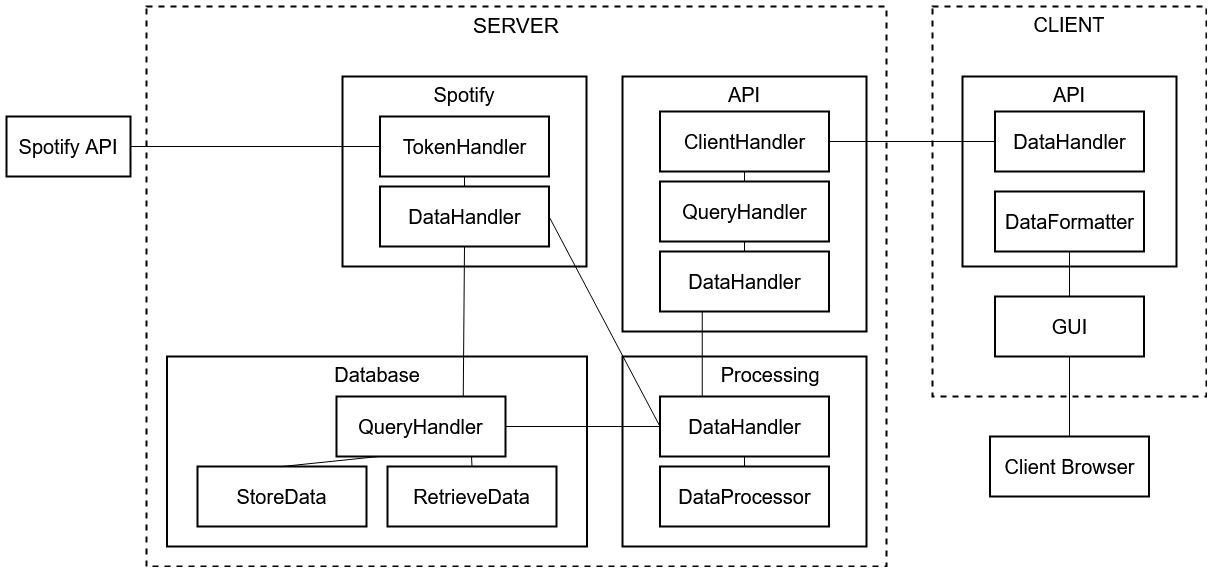
\includegraphics[width=1.2\textwidth]{hla.png}}%
	\caption{High Level Architecture for our system}
	\label{fig:hla}
\end{figure}

\section{Project Outline - JC}

\subsection{Classes}


\subsubsection{Server:}

\hrulefill

\subsubsection{Spotify}
The Spotify class contains all methods for interacting with the Spotify API. This is used in a variety of situations, such as the monitor thread that constantly gets updated information on users or the methods to retrieve the mood information about tracks. 

\subsubsection{Processing}
The Processing class contains all methods for processing the data either saved in the database or pulled from the Spotify API. This processed data is usually then passed to the API and given to the client.

\subsubsection{Database}
The Database class contains all methods and data structures for the database. It includes the data structure for each table within the database, the connection code to the online MongoDB database we are using, and all methods to get and put data to and from the database as needed.

\subsubsection{API}
The API class handles all requests from the client for data. It ensures security using web tokens and sessions, and only allows access to sensitive data when the user connecting successfully authenticates themselves.  


\leavevmode \\

\subsubsection{Client:}

\hrulefill

\subsubsection{GUI}
The GUI will be responsible for displaying the data sent from the server side. It will provide the interface for the user to interact with. The Google Charts API will be used to display the data received from the server as useful, graphically pleasing metrics.

\subsubsection{API}
The API methods will be responsible for interfacing with the server side REST API, both passing data to the server and requesting data from the server.

\subsection{Methods}

\subsubsection{Spotify:}

\hrulefill

\subsubsection{FinaliseAuth}
FinaliseAuth passes the user specific authorisation code to the Spotify API, upon which an access token and a refresh token should be received and returned.

\subsubsection{GetTracksInfo}
GetTracksInfo is a method for getting information (track name, artists, link) from the Spotify API about a list of tracks from their IDs.

\subsubsection{GetAudioFeatures}
GetAudioFeatures is a method for getting audio information (valence, energy, acousticness, instrumentalness, danceability) from the Spotify API about a list of tracks from their IDs.

\subsubsection{GetAccessToken}
GetAccessToken is a method that checks if the access token is still valid. If it is, it simply returns the access token. Otherwise, it uses the refresh token to generate a new access token, and then returns that token.

\subsubsection{DataListener}
The DataListener method runs on a timer from when the server starts running, and every thirty minutes requests all recent tracks that each user in the database has listened to. It then passes these to the database functions to save them into the database.

\subsubsection{GetAllTracks}
GetAllTracks is a method that returns a list of track IDs that contain every song in every playlist the user has, as well as all of their liked songs.

\leavevmode \\

\subsubsection{Database:}

\hrulefill

\subsubsection{AddListenInfo}
AddListenInfo adds a new “listen” to the “Listens” table - it adds a record for each track that a user has recently listened to, including the track’s ID and the user’s ID.

\subsubsection{GetListenInfo}
GetListenInfo gets all tracks that a user has listened to within a specified time period.

\subsubsection{AddUser}
AddUser adds a user to the “Users” table.

\subsubsection{GetUsers}
GetUsers gets all users from the “Users” table.

\subsubsection{GetAuthToken}
GetAuthToken gets the Spotify API auth token for a given user.

\subsubsection{GetRefreshToken}
GetRefreshToken gets the Spotify API refresh token for a given user.

\subsubsection{UpdateAuthToken}
UpdateAuthToken modifies the Spotify API auth token for a given user.

\subsubsection{CheckLoginDetails}
CheckLoginDetails checks that, given a username, such a user exists in the “Users” table, and given a hashed password, a hash exists in that user record that is the same.

\subsubsection{CheckIfUserExists}
CheckIfUserExists checks if a given username already exists in the database.



\leavevmode \\

\subsubsection{Processor:}

\hrulefill

\subsubsection{SortUserSongs}
The SortUserSongs method uses the GetAllTracks method to get all of a user’s tracks, before using the GetTracksInfo method to get those tracks’ names and artists, and then the GetAudioFeatures method to get those tracks’ audio features. Each track is then classified as a specific mood using the Classify method and is returned through an API call.

\subsubsection{ProcessRecentTracks}
ProcessRecentTracks uses the GetListenInfo method from the database to get all recently listened to tracks, before using the GetTracksInfo method to get those tracks’ names and artists, and then the GetAudioFeatures method to get those tracks’ audio features. Each track is then classified as a specific mood using the Classify method and is returned through an API call.

\subsubsection{Classify}
The Classify method looks at the audio features of a song and classifies it as a specific mood using a mood defining algorithm.


\leavevmode \\

\subsubsection{API:}

\hrulefill

\subsubsection{Login}
The Login API endpoint is given a username and password from the client, and uses the CheckLoginDetails method in the database to confirm that a user is valid. If it is, a web token is generated and sent as a cookie to the user, creating a login session for the client.

\subsubsection{Register}
The Login API endpoint is given a username and password from the client, and uses the CheckIfUserExists method in the database to confirm that no user exists with that name. If they do, “false” is sent back, alerting the client that a user already exists with that username. Otherwise, the AddUser method in the database is ran, with the username and password given.

\subsubsection{YesterdayMood}
The YesterdayMood API endpoint uses the ProcessRecentSongs method to get a list of songs that the user listened to in the last day, information about each song and a mood classification for each song.

\subsubsection{MonthMood}
The MonthMood API endpoint uses the ProcessRecentSongs method to get a list of songs that the user listened to in the last month, information about each song and a mood classification for each song.

\subsubsection{Callback}
The Callback API endpoint is used exclusively for Spotify to return an authorisation code for a given user after that user connects their Spotify account to our system. It then uses the UpdateAuthToken method in the database.

\subsubsection{GetTracks}
The GetTracks API endpoint uses the GetAllTracks method and returns that data, for use with the timeline on the front end.

\subsubsection{MoodClassification}
The MoodClassification API endpoint uses the SortUserSongs method and returns that data, for use with the mood charts on the front end.


\section{Sequence Diagram - TD} 

Figure \ref{fig:seqdia} shows the normal path a user will take through the system, it first checks for a valid login, or allows the user to create an account (See functional 1.2, 1.3, 1.4, 1.5, 4.1, 4.3, non-functional 4.2). Once their credentials have been validated the system connects to their Spotify account and collects and analyses their song data, this in then stored in the database (See functional 2.1, 2.2, 3.1, 3.2, 3.5, 4.2). This data can then be displayed to the user in a variety of ways (See functional 4.4, 4.5, 4.6, 4.7, 4.8, non-functional 5.1)

\begin{figure}[h]
	\centering
	\makebox[\textwidth][c]{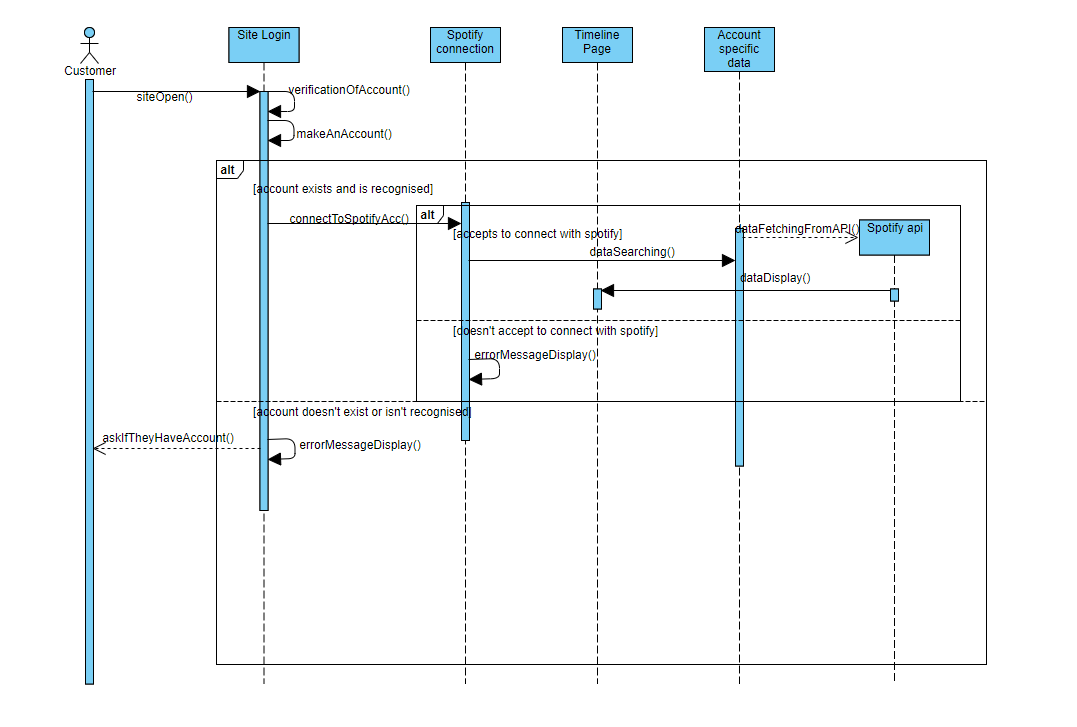
\includegraphics[width=1.2\textwidth]{seq-dia.png}}%
	\caption{Sequence Diagram for our system}
	\label{fig:seqdia}
\end{figure}

\section{Class Diagram - AG}

Figure \ref{fig:classdia} contains almost 2 separate sets of classes, Server and Client. The server classes handle things on the server side, such as storing and receiving from the database, accessing, retrieving and processing Spotify data. The client mostly contains the GUI which is responsible for formatting and displaying data in interesting ways for the user, showing their mood over a day, month etc. The connecting classes are ServerHandler and API and these handle the sending and receiving of data between client and server. So for example if user wishes to see their mood over the last day, the client passes a request to the server handler in which it passes it to the API which handles the request and calls the getListenInfo function and can return to the server handler in which returns it to the GUI. In reference to the relationships between the classes, the server only exists as one entity but will create new instances/threads of the other classes for each client connected. Therefore, the server has a 1 to (possible many) relationship with the 4 server side classes. While the client has a 1 to 1 relationship with the GUI and ServerHandler.

\begin{figure}[h]
	\centering
	\makebox[\textwidth][c]{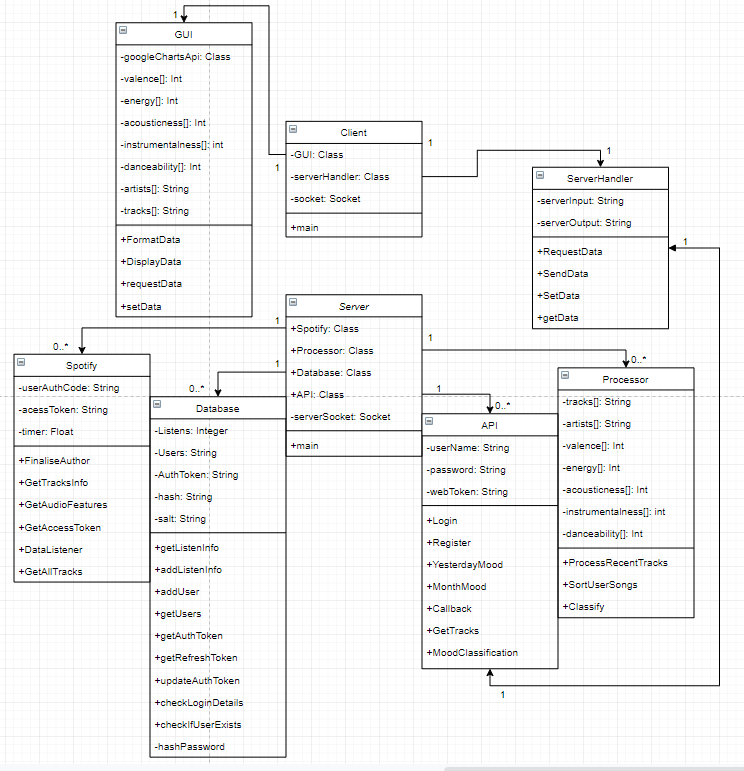
\includegraphics[width=1.2\textwidth]{classdia.png}}%
	\caption{Complete Class Diagram for our system}
	\label{fig:classdia}
\end{figure}

\section{Use Case Diagrams - FD}

There are not many use cases for our program. All of the data entry is automatic so there are no use cases that allow for the user to edit their data. This means we end up with a small number of use case scenarios, which helps to simplify user experience design (See non-functional 5.1)

Figure \ref{fig:usecase1} shows the typical path a user would take when logging in, should they not have an account then they would have to follow figure \ref{fig:usecase2} to create one first and then they can view their data, following figure \ref{fig:usecase3}

Both figures \ref{fig:usecase1} and \ref{fig:usecase2} have corresponding state machine model which can be seen in the next section

\begin{figure}[h]
\centering
\begin{subfigure}{\textwidth}
	\centering	
	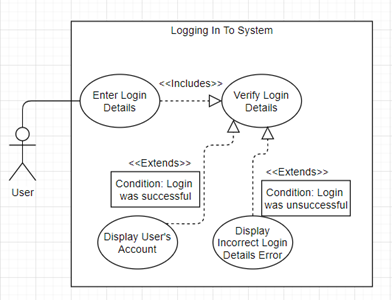
\includegraphics[width=0.5\linewidth]{usecase1.png}
	\caption{Use Case Scenario 1}
	\label{fig:usecase1}
\end{subfigure}
\begin{subfigure}{\textwidth}
	\centering
	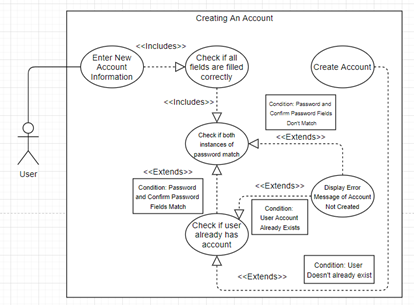
\includegraphics[width=0.6\linewidth]{usecase2.png}
	\caption{Use Case Scenario 2}
	\label{fig:usecase2}
\end{subfigure}
\begin{subfigure}{\textwidth}
	\centering
	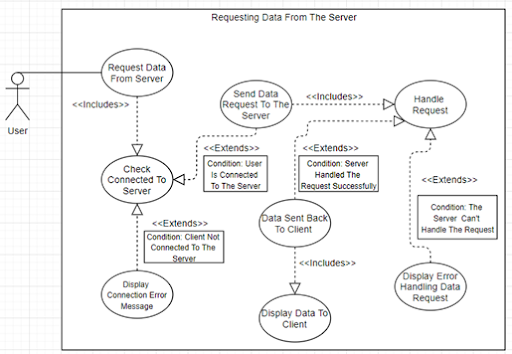
\includegraphics[width=0.6\linewidth]{usecase3.png}
	\caption{Use Case Scenario 3}
	\label{fig:usecase3}
\end{subfigure}

\caption{Different Use Case Scenarios}
\label{fig:usecase}

\end{figure}

\section{State Machine Diagrams - AG}

Figure \ref{fig:statemach1} shows the login state diagram, for use case \ref{fig:usecase1}. The  user enters in username and password on client side and this is sent to the server which first checks if the username exists in the database, if so then prepends the salt stored in that record to the given password and hashes it. If the passwords match then access is granted and they have successfully logged in (See functional 1.1, 1.2, 1.3, 1.5, 4.3 and non-functional 4.2). If the password or username don’t match then it prints an error and starts again at the login page. 

Figure \ref{fig:statemach2} shows the process the system goes through for getting the users data from Spotify and storing it. First the system gets authorisation from the user to allow us to access their account (See functional 2.1, 4.2, non functional 4.3), this gives us an access token which allows us to access their account in future (non-functional 4.2). It then gets all the songs from their library, categorises these into moods and stores them (See functional 2.2, 3.1, 3.2, 4.2). It will then continuously check what the user is listening to, and add any new songs along with the timestamp and mood to the database (See functional 2.2, 3.2, 3.5). This provides the data necessary for functional requirements 4.4, 4.5, 4.6, 4.7, 4.8.

\begin{figure}[h]
\centering
\makebox[\textwidth][c]{
\begin{subfigure}{0.5\textwidth}
	\centering	
	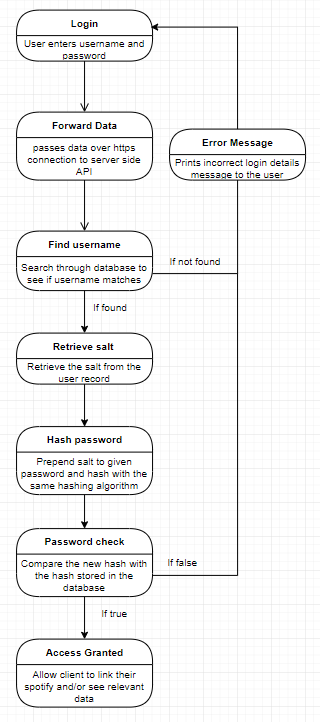
\includegraphics[width=1\linewidth]{statemach1.png}
	\caption{State Machine Model for \ref{fig:usecase1}}
	\label{fig:statemach1}
\end{subfigure}%This Removes the space after these
\begin{subfigure}{0.5\textwidth}
	\centering	
	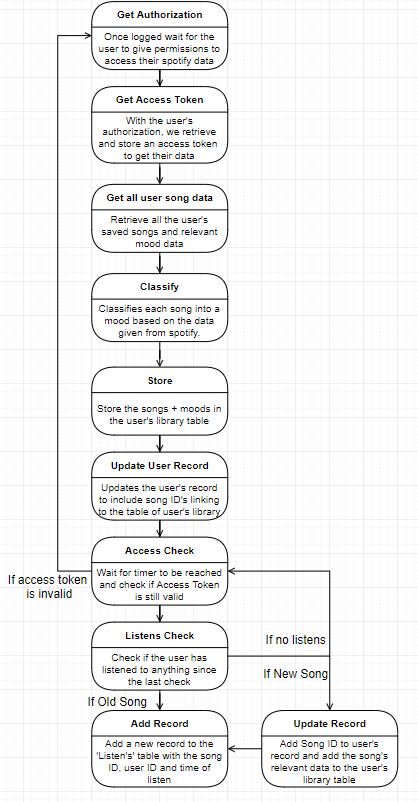
\includegraphics[width=1.2\linewidth]{statemach2.png}
	\caption{State Machine Model for \ref{fig:usecase2}}
	\label{fig:statemach2}
\end{subfigure}
}

\caption{State Machine Models for different Scenarios}
\label{fig:statemach}

\end{figure}

\chapter{Testing}

We performed testing at the end of every sprint. Each sprint looked to build upon the last one (see dependency matrix, figure: \ref{fig:depmat}), so we started with being able to interact between the Server and Client and then moved up to handling accounts and Spotify then finally the user facing front end. This ensured that items that were heavily depended on were done first. This made scaling back our project for COVID-19 as we scaled back items which were less necessary and therefore depended on and we ended up not having to remove any requirements that had already been done. This also made later testing easier as it allows us to incrementally test a larger and larger system, whilst being sure that some parts of it work correctly, rather than having to test all of a large system at once. 

\section{Testing Plans - JC}

All evidence of testing can be found in appendix \ref{test}\\
\textbf{Specification Statement:} F - Functional\quad\quad NF - Non-Functional\\
\textbf{Type:} N - Normal\quad\quad  E - Erroneous\quad\quad  B - Boundary \quad \quad PF - Post-fixing\\
\textbf{Result:} F - Fail\quad\quad  P - Pass

\begin{longtable}{| p{0.4cm} | p{1.8cm} | p{0.7cm} | p{6.5cm} | p{4.5cm} | p{0.5cm}|}
\endfirsthead
\endlastfoot

\multicolumn{5}{c}{\textit{Continued from last page}}
\endhead

\multicolumn{5}{c}{\textit{Continued on next page}} 
\endfoot

\hline
\textbf{N.} & \textbf{Spec. } & \textbf{Typ.} & \textbf{Action} & \textbf{Expected Results}  & \textbf{Re.}\\
\hline
\multicolumn{6}{|c|}{\textit{\textbf{Sprint 1}}} \\
\hline

1&F 1.1&N&Load Login/Register page (\url{http://csed-server.herokuapp.com/})&Login/Register page displays.&P\\ \hline
2&F 1.1&N&Click the “No account? Register here.” Button twice.&The form swaps from the Login form to the Register and then back to the Login form.&P\\ \hline
3&F 1.1, 1.2, 1.3, 1.4, 4.1&N&Go to the Register form and enter: Username: “testAccount”, Password: “password123”, Repeat: “password123”, Click “Register”&The form should close, and the window should redirect to Spotify’s login portal.&P\\ \hline
4&F 1.1, 1.2, 1.3, 1.4, 4.1&E&Go to the Register form and enter: Username: “testAccount2”, Password: “password123”, Repeat: “password12”, Click “Register”&Error message displays: “Passwords do not match.”&P\\ \hline
5&F 1.1, 1.2, 1.3, 1.4, 4.1&E&Go to the Register form and enter: Username: “”, Password: “password123”, Repeat: “password123”, Click “Register”&Error message displays: “You may not leave the username field empty.”&P\\ \hline
6&F 1.1, 1.2, 1.3, 1.4, 4.1&E&Go to the Register form and enter: Username: “testAccount”, Password: “password12”, Repeat: “password12”, Click “Register”&Error message displays: “That username is already taken.”&P\\ \hline
7&F 1.1, 1.2, 1.3, 1.4, 4.1&E&Go to the Register form and enter: Username: “testAccount2”, Password: “”, Repeat: “”, Click “Register”&Error message displays: “You may not leave the password field empty.”&P\\ \hline
8&F 1.1, 1.2, 1.3, 1.4, 4.1&B&Go to the Register form and enter: Username: “ ” (space character), Password: “password123”, Repeat: “password123”, Click “Register”&Error message displays: “You may not leave the username field empty.”&F\\ \hline
9&F 1.1, 1.2, 1.3, 1.4, 4.1&B, PF &Go to the Register form and enter: Username: “  ” (two space characters), Password: “password123”, Repeat: “password123”, Click “Register”&Error message displays: “You may not leave the username field empty.”&P\\ \hline
10&F: 1.4, 4.1&N&Check database for account “testAccount”&Account “testAccount” is in database ‘Users’ table&P\\ \hline
11&F: 1.2, 1.3, 1.4, 4.1&E&Check database for account “testAccount2”&Account “testAccount2” is not in database ‘Users’ table&P\\ \hline
12&F: 1.1, 1.2, 1.3, 1.4, 4.1, 4.3&N&Go to the Login form and enter: Username: “testAccount”, Password: “password123” Click “Login”&The form should close, and the window should redirect to the landing page.&P\\ \hline
13&F: 1.1, 1.2, 1.3, 1.4, 4.1, 4.3&E&Go to the Login form and enter: Username: “testAccount”, Password: “password12” Click “Login”&Error message displays: “Incorrect username or password.”&P\\ \hline
14&F: 1.1, 1.2, 1.3, 1.4, 4.1, 4.3&E&Go to the Login form and enter: Username: “testAccount2”, Password: “password123”, Repeat: “password12”, Click “Login”&Error message displays: “Incorrect username or password.”&P\\ \hline
15&F: 1.1, 1.2, 1.3, 1.4, 4.1, 4.3&E&Go to the Login form and enter: Username: “testAccount”, Password: “”, Click “Login”&Error message displays: “Incorrect username or password.”&P\\ \hline
16&F: 2.1, 2.2, 4.2&N&Check database for account “testAccount” & Random string should be generated and stored in database ‘Users’ table ‘auth\_key’ field after being sent as a unique ID for Spotify’s callback request&P\\ \hline
17&F: 2.1, 2.2, 4.2&N&Login to Spotify using the previously opened Spotify login portal. Check database for account “testAccount”&User should be redirected to the landing page. Previously generated random string should be replaced with an authorisation key from Spotify&P\\ \hline
18&F: 2.1, 2.2, 4.2&N&Check database for account “testAccount”&A temporary access key should have been generated by the backend, storing a refresh token from Spotify in the database ‘Users’ table ‘refresh\_token’ field.&P\\ \hline

\multicolumn{6}{|c|}{\textit{\textbf{Sprint 2}}} \\
\hline

19&F: 1.5 NF: 4.2&N&Go to the Register form and enter: Username: “hashTest”, Password: “password123”, Repeat: “password123”, Click “Register”&The form should close, and the window should redirect to Spotify’s login portal.&P\\ \hline
20&F: 1.5 NF: 4.2&N&Check database for account “hashTest”&Account “hashTest” is in database ‘Users’ table, password is hashed.&P\\ \hline
21&F: 1.2, 1.5 NF: 4.2&N&Go to the Login form and enter: Username: “hashTest”, Password: “password123”, Click “Login”&The form should close, and the window should redirect to the landing page.&P\\ \hline
22&F: 1.2, 1.5 NF: 4.2&E&Go to the Login form and enter: Username: “hashTest”, Password: “password12”, Click “Login” &Error message displays: “Incorrect username or password.”&P\\ \hline
23&F: 1.2 NF: 4.2&N&Go to the Login form and enter: Username: “hashTest”, Password: “password123”, Click “Login”, Reload landing page &The form should close, and the window should redirect to the landing page. The landing page should load again when reloaded.&P\\ \hline
24&F: 1.2 NF: 4.2&E&Go to the Login form and enter: Username: “hashTest”, Password: “password123”, Click “Login”, Wait 30 minutes (or go to incognito mode), Reload landing page&The form should close, and the window should redirect to the landing page. Upon reload, the landing page should be replaced by an error message: “You need to log in.”&P\\ \hline
25&F: 1.2 NF: 4.2&E&Go to the landing page: https://csed-server.herokuapp.com/landing&An error message should display: “You need to log in.”&P\\ \hline
26&F: 1.2 NF: 4.2&E &Go to an API endpoint: http://csed-server.herokuapp.com/api/moodCount&An error message should display: “You need to log in.”&P\\ \hline
27&F: 2.1, 2.2, 3.1, 3.2, 3.5, 4.4, 4.8 NF: 4.2, 4.3, 6.3&N&Go to the Login form and enter: Username: “joe”, Password: “test”, Click “Login”&The form should close, and the window should redirect to the landing page. The daily mood graph should be visible and filled in.&P\\ \hline
28&F: 2.1, 2.2, 3.1, 3.2, 3.5, 4.8 NF: 4.2, 4.3, 6.3&N&Go to the Login form and enter: Username: “joe”, Password: “test”, Click “Login”, Go to an API endpoint: http://csed-server.herokuapp.com/api/dayMood?date= 4/3/2020&The form should close, and the window should redirect to the landing page. At the API endpoint, JSON data should be presented.&P\\ \hline
29&F: 2.1, 2.2, 3.1, 3.2, 4.5 NF: 4.2, 4.3, 6.3&N&Go to the Login form and enter: Username: “joe”, Password: “test”, Click “Login”&The form should close, and the window should redirect to the landing page. The library mood classification pie chart should be visible and filled in.&P\\ \hline
30&F: 2.1, 2.2, 3.1, 3.2, 3.5, 4.5 NF: 4.2, 4.3, 6.3&N&Go to the Login form and enter: Username: “joe”, Password: “test”, Click “Login”, Go to an API endpoint: http://csed-server.herokuapp.com/api/moodCount&The form should close, and the window should redirect to the landing page. At the API endpoint, JSON data should be presented.&P\\ \hline

\multicolumn{6}{|c|}{\textit{\textbf{Sprint 3}}} \\
\hline

31&F: 2.1, 2.2, 3.1, 3.2, 3.5, 4.6, 4.8 NF: 4.2, 4.3, 6.3&N&Go to the Login form and enter: Username: “joe”, Password: “test”, Click “Login”&The form should close, and the window should redirect to the landing page. The timeline table should be visible and filled in.&P\\ \hline
32&F: 2.1, 2.2, 3.1, 3.2, 3.5, 4.6, 4.8 NF: 4.2, 4.3, 6.3&N&Go to the Login form and enter: Username: “joe”, Password: “test”, Click “Login”, Go to the timeline table and scroll down within it&The form should close, and the window should redirect to the landing page. The timeline table should be visible and filled in. The timeline table should update as the user scrolls down, filling in previous days.&P\\ \hline
33&F: 2.1, 2.2, 3.1, 3.2, 3.5, 4.8 NF: 4.2, 4.3, 6.3&N&Go to the Login form and enter: Username: “joe”, Password: “test”, Click “Login”, Go to an API endpoint: http://csed-server.herokuapp.com/api/getRecentTracks ?date=5/4/2020&The form should close, and the window should redirect to the landing page. At the API endpoint, JSON data should be presented.&P\\ \hline
34&F: 2.1, 2.2, 3.1, 3.2, 3.5, 4.8 NF: 4.2, 4.3, 6.3&N&Go to the Login form and enter: Username: “joe”, Password: “test”, Click “Login”, Go to an API endpoint: http://csed-server.herokuapp.com/api/getRecentTracks ?date=5/1/2020&The form should close, and the window should redirect to the landing page. At the API endpoint, JSON data should be presented. The data should be different to the previous test.&P\\ \hline
35&F: 2.1, 2.2, 3.1, 3.2, 3.5, 4.8 NF: 4.2, 4.3, 6.3&N&Go to the Login form and enter: Username: “joe”, Password: “test”, Click “Login”&The form should close, and the window should redirect to the landing page. The top songs table should be visible and filled in.&P\\ \hline
36&F: 2.1, 2.2, 3.1, 3.2, 3.5, 4.8 NF: 4.2, 4.3, 6.3&N&Go to the Login form and enter: Username: “joe”, Password: “test”, Click “Login”, Go to an API endpoint: http://csed-server.herokuapp.com/api/topTen&The form should close, and the window should redirect to the landing page. At the API endpoint, JSON data should be presented.&P\\ \hline
37&F: 2.1, 2.2, 3.1, 3.2, 3.5, 4.4, 4.8 NF: 4.2, 4.3, 6.3&N&Go to the Login form and enter: Username: “joe”, Password: “test”, Click “Login”, Select a new date for the daily mood graph (5/1/2020)&The form should close, and the window should redirect to the landing page. The daily mood graph should be visible and filled in. The daily mood graph should change when the date is changed on it.&P\\ \hline
38&F: 2.1, 2.2, 3.1, 3.2, 3.5, 4.4, 4.8 NF: 4.2, 4.3, 6.3&E&Go to the Login form and enter: Username: “joe”, Password: “test”, Click “Login”, Select a future date for the daily mood graph (5/10/2020)&The form should close, and the window should redirect to the landing page. The daily mood graph should be visible and filled in. The future date should not be selectable.&P\\ \hline
39&F: 2.1, 2.2, 3.1, 3.2, 3.5, 4.8 NF: 4.2, 4.3, 6.3&N&Go to the Login form and enter: Username: “joe”, Password: “test”, Click “Login”, Go to an API endpoint: http://csed-server.herokuapp.com/api/dayMood?date= 5/4/2020&The form should close, and the window should redirect to the landing page. At the API endpoint, JSON data should be presented.&P\\ \hline

\end{longtable}


\begin{comment} OLD
\begin{center}

\begin{longtable}{| p{2.5cm} | p{6cm} | p{2cm} | p{2cm} | p{2.5cm} | }

\hline
\textbf{Name} & \textbf{Description} & \textbf{Data Type} & \textbf{Actual Data} & \textbf{Expected Outcome} \\
\hline

\endfirsthead

\endlastfoot

\multicolumn{5}{c}{\textit{Continued from last page}}
\endhead

\multicolumn{5}{c}{\textit{Continued on next page}} 
\endfoot

\multicolumn{5}{|c|}{\textbf{Sprint 1}} \\
\hline
\multicolumn{5}{|l|}{\textbf{\textit{Acquiring data from Spotify}}} \\
\hline
Authorise Spotify user account&
Program should be able to request access to a user’s Spotify account and store the returned access token for later use&
Valid Spotify username / password combination&&
Valid Spotify access Token\\
\hline
Data successfully obtained from Spotify&
Show that data collection from Spotify functions correctly, this does not include the account authorisation stage, but rather that the server can obtain data form Spotify, what data does not matter as long as it is the same as requested&
Valid access token and API query&&
Spotify returns specified data\\
\hline
\multicolumn{5}{|l|}{\textbf{\textit{Login Pages}}} \\
\hline
Login and Create Account pages&
Login and Create Account pages are sent to the user and are visually functional when the user requests them using http&
Page URLS&&
Server should send the pages through http\\
\hline
Create Account successfully creates account when valid account data is provided&
Create Account page successfully sends correct data to the server, allowing it to correctly create accounts, this must also contain all of the necessary data, and return a correct Account Creation page and message, when all the data sent is valid&
Valid and not already used user data&&
Server should send a success message or send the user to an account created page\\
\hline
Create Account correctly displays error message when invalid account data is provided&
Create Account page throws an error when the user enters data which is not valid or uses data which has been already used and does not overwrite or data the already existing data&Invalid or already used user data&&
Server should stay on page and send an error message to the user, telling them what caused the error\\
\hline
Login is successful when correct account credentials are entered&
Login page should log the user in when they enter the correct username / password pair&
Valid username / password combination&&
The user is logged in, redirecting to a landing page\\
\hline
Login is unsuccessful when incorrect credentials are entered&
Login should fail when the user enters credentials which are not valid, the page, should not give away whether an account exists with the given username / email but rather a generic failed message in order to comply with security best practises&
Invalid username / password combination&&
The user is not logged, however is left on the log in page with a generic error message\\
\hline
\multicolumn{5}{|c|}{\textbf{Sprint 2}} \\
\hline
\multicolumn{5}{|l|}{\textbf{\textit{Security}}} \\
\hline
Passwords are hashed and stored&
Passwords are hashed and stored as outlined in password storage guidelines (Research: 3.3): Salted and hashed (argon2 was recommended), with only these stored in databased&
Register account with valid credentials, check database to ensure plaintext password not stored&
N/A - Can be checked on database&
Password stored in database will be hashed, stored alongside the salt\\
\hline
Hash salts should be safely generated&
Password salts should be generated in such a way which makes them hard to guess (ex. Not generated based on other account info, or using Cs generator without a seed)&Register account with valid credentials, check database to show&
N/A - Can be checked on database&
List of randomly generated salts, (Note that even easy to guess salts will appear random, so code review is best to established this has been met)\\
\hline
\multicolumn{5}{|l|}{\textbf{\textit{Security}}} \\
\hline
Server is able to retrieve song characteristics from Spotify&
Server can gather characteristics on a song using the Spotify API, these can then be used in order to classify the songs mood&
Song ID passed to Spotify&
https://api.spotify.com/v1/audio-analysis/51xPLClVr9DDGwrtnFc6DF&
Relevant data for song (Sally Cinnamon, The Stone Roses)\\
\hline
Server is able to characterise songs&
Server can characterise any given song based on the statistics provided by the Spotify API&
Song data provided by Spotify&
N/A - can be checked through API&
All songs users have in library should be categorised\\
\hline
Server tracks users listening habits&
Server periodically checks to see what the client has listened to and then and adds these to the database&
Check through API (See API Section)&
N/A - can be checked through API&
Users listened to songs should appear\\
\hline
Server tracks contents of user’s library&
Server gathers user’s library of songs from the playlists they have&
Check through API (See API section)&
N/A - can be checked through API&
All songs in a user’s playlists should appear\\
\hline
Server characterises user listening habits&
Server should characterise songs the user has listened into moods based on the characteristics of those songs as outlined in mood table (Research: 3.5)&
Check through API (See API section)&
N/A - can be checked through API&
Mood should appear alongside listened songs, these do not have to be perfect but should give a good representation\\
\hline
\multicolumn{5}{|l|}{\textbf{\textit{API}}} \\
\hline
API should show no data if the user is not logged in&
Requests made without a valid auth token should either be turned away or ignored&
Test API pages before logging in&
Try: JOE CORRECT URL PLZ without auth token&
No data will be displayed\\
\hline
API allows for access to categorisation of user songs&
API should provide a method of viewing user data of library (note that this does not have to be the final page with a user facing interface)&
API page link&
JOE CORRECT URL PLZ&
All user data for library and its characterisation should be displayed\\
\hline
\multicolumn{5}{|c|}{\textbf{Sprint 3}} \\
\hline
\multicolumn{5}{|l|}{\textbf{\textit{Frontend Navigtion}}} \\
\hline
Frontend navigation functions correctly&
User can navigate to all of the different pages of the frontend using just the buttons provided&
Website&
<Insert landing page here>&
Page should appear as per design and should be easy to navigate with on-site tools (no manual entering of URLs should be required)\\
\hline
Frontend redirects user if not logged in&
Frontend redirects the user should they try and access pages they do not have access to&
Website&
<Insert landing page here>&
User will be redirected to the login / create account page should they try and access any page which requires account credentials \\
\hline
\multicolumn{5}{|l|}{\textbf{\textit{Security}}} \\
\hline
User should not be able to view / access other users’ data&
Frontend should not expose any user data unless the user is logged into that user account with valid credentials&
Website&
<Insert landing page here>&
User will be shown no data if they do not have valid credentials and should be redirected (see above) \\
\hline
\multicolumn{5}{|l|}{\textbf{\textit{Data Representations}}} \\
\hline
User should be able to view all songs in their library&
Webpage should provide a method for the user to view all the items in their library along with moods and view counts&
Website&
<Insert landing page here>&
User library should be displayed if user has correct login credentials \\
\hline
User should be able to view a timeline of their recently listened to songs&
Webpage should provide a method for the user to view all their recently listened to track in a timeline format&
Website&
<Insert landing page here>&
Timeline of user listens should be displayed if user has correct login credentials \\
\hline
User should be able view statistics on the makeup of their library and listening habits&
Webpage should provide a method for the user to view statistics such as the mood makeup of their library and last day of listening&
Website&
<Insert landing page here>&
Statistics on library and listen makeup should be displayed on page if the user has correct login credentials \\
\hline


\end{longtable}

\end{center}
\end{comment}

\chapter{Conclusion  - SC}

SpotiMy has been a great learning experience for our team and, overall, a success. The final version of our project has met our expectations and the journey of creating it has taught us about organisation, teamwork, self-learning and utilising our sets of skills. SpotiMy is a personal informatics software, which, upon research and development, helps the user understand and classify the songs they listen to, based on the mood the music conveys. It takes raw data from the user’s Spotify account which is then processed into something they can easily understand and reflect upon by the use of graphs and intuitive user interface. 

As any major project, SpotiMy has its strengths and weaknesses. It started as a fun project idea, which took contour in the first weeks of the semester. Upon reflection, the planning stage of our project was vague, our idea not being well-defined. If something could have been done differently about this, assessing everyone’s skills and knowledge at the beginning of the project would have helped assure that everyone would be able to contribute in equal amounts. This would have also been a better guide about what our team was able to create in the most efficient way. 

On the other hand, an advantage was that our set of requirements was constructed concisely, which was useful when building the software as well as tracking our progress. The requirements were updated regularly if any change occurred and this helped make sure there were no misunderstandings. The testing plan was created before developing the software which was useful because we knew exactly what the software was supposed to do. For one of our testing plans, upon feedback of our tutor, we had to break down some of our tests and 
make minor changes, but this did not cause any problems in the end. 

Our design was also successful, giving us an idea of what the user interface was supposed to look like. Drawing diagrams to illustrate this before creating it helped us make sure we would not implement something that we were not happy with. The Class Diagrams, State Machine Diagrams and Use Case Diagrams were useful during the development of the software. They are detailed and clear, making them a great guide to how the software is supposed to function. 

Regarding research, we found plenty of useful articles to base our software on. Although our research was useful, we have created and distributed our questionnaire too late in our development process, therefore we discarded it and we had a low amount of responses. It would have been better If we would have prioritised it in the beginning of our project. In this way we could have used it as a tool to guide us and suggest ways of making our project better and more useful to the target audience. 

The organisation of the team was good, even though there were more people in this semester’s project compared to the project we made in the first semester, the Scrum method helped us greatly. It was a good way of us keeping track of our progress and our meetings. In the first semester we did not use GitHub and did not have a product backlog, which made us far less organised and less adaptable to change. It was hard to keep track of what everyone was doing, and it was hard to estimate the amount of time needed to complete the work, leaving us with a lot of work due before the deadline. 

In this semester, iterative development was a good way of observing the project at different stages. This offered us more freedom and ability to change by reflecting on the previous sprints and thinking about where the project was going along the way. For example, we were able to decide to have a longer sprint during difficult times, so that the work could be finished. The scrum methodology helped us have a better attitude towards our responsibilities as everyone was able to pick a task they wanted to do, and they were supposed to complete it in the time of the sprint. We had deadlines that motivated us to get work done, and we helped each other as a team by reviewing each other’s progress and suggesting improvements in our meetings. 
We learnt to help each other in case someone had questions about their task and to be understanding yet prompt. Because of the workload that needed to be done we also had to pick tasks we were not initially comfortable with, which have helped us with self-development and with the help of our teammates and self-learning, broadening our sets of skills. The two projects helped us understand what working in a team is like and develop our attitude towards working with other people that have a common goal, as well as the advantages of using an agile method. 

We have developed our attitudes towards trying to get involved in new topics and dealing with difficult situations. We had to deal with some of our teammates not being able to participate because of personal issues as well as working remotely. Our original risk assessment helped us as we were prepared and anticipated these situations. To be able to keep working normally even during the Covid19 pandemic, we had online meetings using Teams, used Google Documents for our report so everyone could edit it, GitHub to upload our work and keep track of our progress, and WhatsApp to plan our meetings and communicate outside of them when needed. 

After completing both the projects and being able to compare and reflect on them, we learnt that organisation is a highly important aspect when working in a team or tackling a big project. We were able to observe the advantages of using Scrum, as well as good communication and planning. Completing the two projects was a learning experience that will help us along the way while working in a software developing team.

%Loads bibliography
\bibliography{ref}{}
\bibliographystyle{bathx}

\chapter{Appendix}

\section{Group Contribution Form}

The Group Contribution is at follows:
\begin{itemize}
\item Adam George			06
\item Edward Dunton		10
\item Fraser Dwyer			10
\item Joseph Cryer			10
\item Lance Garcia			02
\item Sam Davidson			06
\item Sam Freeman 			04
\item Sandra-Maria Corradi	08
\item Teodora Dinca    		06
\end{itemize}

Our Group Contribution Form can be seen in figure \ref{fig:gcf}

Lance and Sam Freeman ended up getting lower scores as both were barely seen after sprint 1, and neither contributed any work towards the project after that point, Sam did however contribute more to the project during the period he was around and therefore has been given a higher score

Eddy and Joe contributed the most of the code and for that reason have been given higher scores, Fraser contributed a large amount towards the contents of the report

As the team was unable to meet due to COVID-19 we were unable to sign it and instead had to approve it via teams. As neither Lance nor Sam Freeman were around to communicate during sprint 2 and 3 we were unable to get their approval.

\newpage

\begin{figure}[!h]
	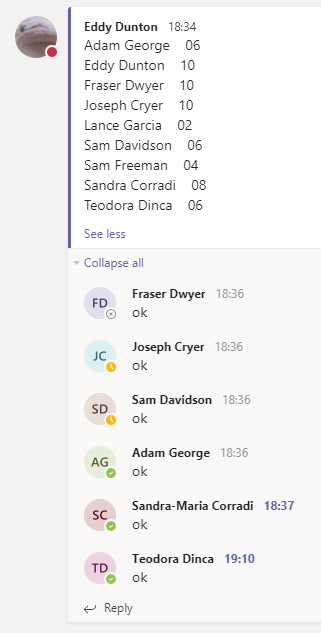
\includegraphics{gcf.png}
	\caption{Group Contribution Form as seen on MS Teams}
	\label{fig:gcf}
\end{figure}

\newpage

\section{Research}
\label{res:res}

\subsection{Prior Research - LG}
\label{res:prior}

This research was performed before the final solution was decided, it was performed by various members then collated by Lance Garcia.\newline

A recurring theme throughout our research into personal informatics is the idea that the user must want to track their data, as well understand how to best make use of the system given to them. \cite{Rapp2014a} suggests that “common users” with little prior experience can suffer from problems with familiarity and motivation with the tracking of their personal data. They go on to suggest factors that affect self-monitoring such as “motivation for change” and “goal-setting feedback and reinforcement” should be kept in mind during the development of the program in order to maximise user interaction with the app. Through the factors given in this article, we should be able to increase the effectiveness of the user monitoring their own data, as well as collect accurate and important data.

This is supported by \cite{Fritz2014} who studied the long-term effects of using personal informatics tracking devices such as Nike’s “FuelBand” which discovered many users experienced a short-term improvement to their health. This was due to the encouragement that users receive on such devices. This highlights the potential for long term health benefits to users that are motivated enough to continue monitoring their data over longer period. While this is not directly applicable to our proposed solution, it provides insight to the effects of personal informatics in the long and short-term. In a similar manner, being able to track what kinds of music make the user happier or focused may provide benefits to them in the long run as they listen to more of that type of music.

The idea of trust in a system is an important concept; a user’s trust in the system is important as that will affect their motivation, and their likelihood of continued use of the system. In the case that the program produces a result that either the user disagrees with or dislikes, this can lead to a loss in trust, and as a result, a loss of interest in the system. To increase this sense of trust, the user should be shown how the data is collected, and to provide them with an understanding of what the data means. In addition to this, meaningful data visualisation and explanation will help to provide this understanding to the user. \cite{Jaimes2013}

\cite{Li2010} mentions five steps for developing personal informatics software being: preparation, collection, integration, reflection, and action.  It should be a conscious decision to integrate these steps into our software as it will enable the users to not only flit back and forth between these stages with ease. This will also allow us to make as much of the program software driven in order to make it more reliable and through reducing the amount that the user must do/understand will help the user to monitor their own data with minimal effort.

\subsection{Security Ethics - AG}
\label{res:secethics}

This research was performed during the production of the product, in order to ascertain ethical guidelines for users to developers to follow when securing user data.\newline

The idea of responsible disclosure is highlighted by \cite{2010a} which describe it as: “researchers who uncover a flaw don't go public until the system's developer has had a chance to fix it”.  This is of note as this not only provides the developer’s with time to patch their system, but also to prevent the public from losing trust in said system.  Responsible disclosure is a “community accepted” protocol, so while it may not be mandatory for researchers and developers to follow through, it is in the best interest of most companies to align themselves by it.

A growing ethical concern is the phenomenon of social networks.  With the group project being involved with music apps, which are commonly linked to users’ social media accounts, this is of important note.  The issue comes in the place of a lack of “central command” which is compounded by anonymity, as well as virtual/multiple personalities.  This brings in a wide range or social and ethical issues with the use of social networking, examples of this being cyberbullying, cyberstalking, and cyber-harassment.  According to a survey taken by i-SAFE, more than 53\% of children admit to having been abusive over the internet, with 42\% having admitted to being victims of said abuse \cite{iSAFE2004}. In addition to this, the use of social networking has led to internet addiction being a clinical disorder.  Users that are extroverted/unselfconscious, shy, or narcissistic \cite{Kizza2016} tend to have higher usages of social networking applications.  


\subsection{Hashing and Password Storage - AG}
\label{res:passsec}

This research was performed during the production of the product, in order to ascertain security guidelines for the storing of passwords.\newline

Without any sort of hashing or protection a database breach could lead attacks to obtaining users usernames and passwords in plaintext, allowing them to access users accounts on this or any other service which they used the same credentials for in a credential stuffing attack, one of the most common styles of cyber-attacks \cite{OWASP2020}. Hashing turns a plaintext password into a random string of characters which cannot be reversed, instead, when a user enters their password it is hashed, and the 2 hashes are compared.

A common principle to follow in system security is Shannon's Maxim: "one ought to design systems under the assumption that the enemy will immediately gain full familiarity with them" \cite{Shannon1949}.This essentially means that a system shouldn’t be secure through obscurity, i.e even if the attackers know the algorithms/protocols that encrypt the data, they still shouldn’t be able to break the security. In theory hashing can be brute forced with current technology, however, the necessary computing power is not readily available at this moment, but, this may change in the near future. Another common approach to breaking hashes is to use a lookup table which stores the most commonly used passwords along with their hashes, which makes these passwords trivial to break. For this reason, hashing alone is insufficient for password security. \cite{Tsudik1992}

For this reason salts are used, which are randomly generated strings added to the password before hashing when the password is created, the salt is stored in the database alongside the password. This helps prevent against these pre-calculated hash tables because the hacker has to then recalculate these tables for each user they wish to hack into as they will have their own unique salt with them which makes these attacks more costly. Brute force attacks can never be fully stopped but using a modern hashing algorithm can make it more expensive for the attacker, as these focus less on speed, but instead flexibility, for example, argon2 has parameters such as memory size, iteration count, parallelism and salt length which can be adjusted to make the hash more (or less) complex making it more expensive to brute force as more resources can be required to perform a hash \cite{Biryukov2016}. For these reasons we recommend the use of Argon2 over other modern algorithms such as the SHA family or Bcrypt.

\subsection{Ethics of Data Storage - SD}
\label{res:datastor}

This research was performed during the production of the product, in order to ascertain guidelines for the storage and usage of user data.\newline

Data today is something that is a key asset to companies and the day to day operations in the world. Behind it, there are many legal and ethical aspects which are important to the privacy and safety of the users who give up their data. To understand what the responsibilities are we would look into the Association of Computing Machinery’s Code of Ethics and Professional Conduct. In section 1.2 it is considered a general ethical principle to “avoid harm”, harm meaning any negative or unfair and significant consequences \cite{ComputingMachineryACM2018}. In terms of the data that we hold, if we pass on or give up the data to anyone else other than just for our program then we would potentially be harming the user, who have put their trust in us using their data. One example of a large company misusing information is the Facebook-Cambridge Analytica scandal in 2018. This is when Facebook allowed enough data for the political consulting company Cambridge Analytica to create psychological profiles on 70.6 million US citizens during the US presidential election in 2016 \cite{Horwitz2018}. They used this collected data to create political regressive models on users for advertisement purposes, this led to predicting users’ personalities which were then presented with adverts which promoted certain political agendas, influencing voters through micro-targeted advertisements \cite{Rathi2019}. This incident was considered illegal and unethical as they broke the British law, harvesting almost all data without explicit consent \cite{ASNC2018}. As we are dealing with personal information as well, it is very possible that the data we collect could create psychological profiles. This must be avoided, and data collected will be deleted after its intended use.

When considering the ethical concerns for storing and analysis of data, there is none when the user has given their expressed consent where they are informed fully of what the data will be used for. Additionally, with accordance to the GDPR, which looks for fairness and transparency, if a user wishes to retract their information from being used then we must return or delete the data. We must also only use the data we collect for the use we have clearly said to the user


\subsection{Song attributes and mood - SC}
\label{res:mood}

This resesarch was performed during the production of the product, in order to ascertain the relationship between characteristics of songs and their moods.\newline

The Mood Table was created based on Thayer’s mood mode, Figure \ref{fig:thayermoodmodel}, which considers the energy and the valence of a song to determine basic moods. “In most existing methods of music mood classification, the moods of songs are divided according to psychologist Robert Thayer’s traditional model of mood. The model divides songs along the lines of energy and stress, from happy to sad and calm to energetic, respectively (Bhat et al 359). The eight categories created by Thayer’s model include the extremes of the two lines as well as each of the possible intersections of the lines (e.g. happy-energetic or sad-calm). [...]” \cite{Nuzzolo2015}. The mood table makes use of this information by working with data provided by Spotify, the energy and the valence. The model has been refined by taking into consideration another 3 variables, acousticness, instrumentalness and danceability. These are considered attributes that create subsets of the already existing moods, making them more specific and detailed. High acousticness and instrumentalness can be used to determine a song is motivational or good for concentration, while danceability can help determine how lively a song is. 

This led us to the following matrix, here all values must align with the required values for a song to be categorised as a certain mood.
Required values:
\begin{itemize}
\item 'n' - Neutral - Value must be between 0.4 and 0.6
\item '+' - Positive - Value must be above 0.6
\item '-' - Negative - Value must be below 0.4
\item '/' - Non-dependant - Value does not matter
\end{itemize} 


\begin{longtable}{| p{5cm} | p{2.5cm} | p{2.5cm} | p{2.5cm} |  p{2.5cm} |}
\hline
\textbf{Mood} & \textbf{Valency} & \textbf{Energy} & \textbf{Acoutstic} & \textbf{Danceability} \\
\hline
\endfirsthead

\endlastfoot

\multicolumn{5}{c}{\textit{Continued from last page}}
\endhead

\multicolumn{5}{c}{\textit{Continued on next page}}
\endfoot

Neutral		&n&n&/&/\\
Happy			&+&n&/&/\\
Sad			&-&n&/&/\\
Calm			&n&-&/&/\\
Energetic		&n&+&/&/\\
Exuberance		&+&+&/&/\\
Lively			&+&+&/&+\\
Joyful			&+&n&/&+\\
Contentment		&+&-&/&/\\
Relaxation		&+&-&/&/\\
Frantic		&-&+&/&/\\
Depressing		&-&-&/&/\\
Melancholic		&-&-&+&/\\
For Concerntraion	&n&-&+&/\\
Motivational		&n&+&+&/\\
\hline
\end{longtable}

\subsection{Questionnaire - SC}
\label{res:quest}
A questionnaire has been used to gather data about the correlation between people’s moods and their music listening habits. Of our 24 responses we found out that around 90\% of people agree with the statement “My listening habits change based on my mood” while 40\% out of them strongly agree. Furthermore, 70\% of people state that music plays a big role in their lives, while 60\% of them think the music they listen to helps them understand themselves more. Most people stated that they listen to music at least 4 days a week, while a big part of them (65\%) listen to music daily. Generally, people listen to music a couple of hours a day, while some listen to music all the time, or less than an hour a day. Music seems to help people deal with their emotions \ref{fig:question-moods} and most people seem to use Spotify as their main music app \ref{fig:question-format}. We have also asked if there were any features, they wished music apps included. A couple of responses addressed the way songs are recommended to them and organised, stating that they wished the recommended songs would fit the way they are feeling at the time more, and that they would like to be able to have direct access to songs they listened to before. Other responses talked about displaying lyrics and tools to help the user recognise songs more easily. This information has strengthened the ideas our research provided and has helped us gain a better understanding of how music affects people’s moods. It has prompted us to create an app that helps people track their moods based on what they listen to on Spotify.

\newpage

\section{Figures}

\begin{figure}[h]
	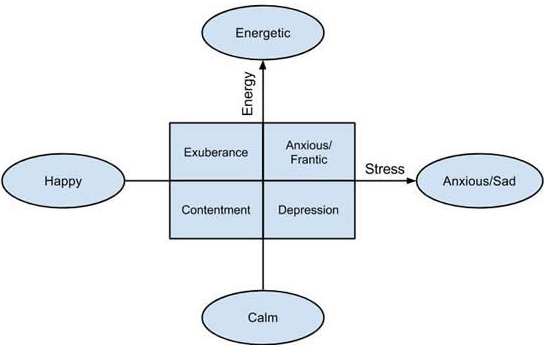
\includegraphics[width=\linewidth]{thayer-mood-model.png}
	\caption{Thayer Mood Model}
	\label{fig:thayermoodmodel}
\end{figure}

\newpage

\begin{figure}[h]
\centering
\begin{subfigure}{\textwidth}
	\centering	
	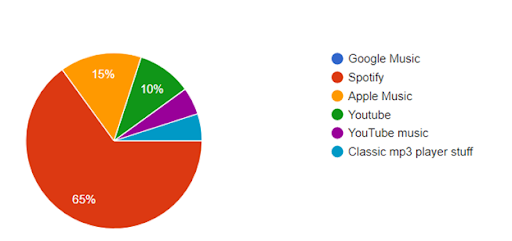
\includegraphics[width=0.9\linewidth]{question-moods.png}
	\caption{Do moods help you express or cope with different emotions and moods?}
	\label{fig:question-moods}
\end{subfigure}
\begin{subfigure}{\textwidth}
	\centering
	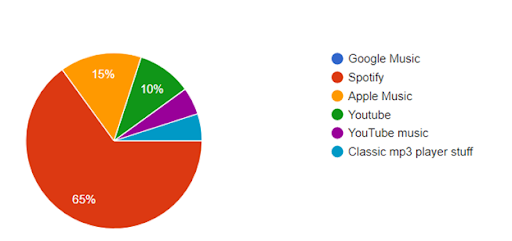
\includegraphics[width=0.9\linewidth]{question-format.png}
	\caption{What music application do you prefer?}
	\label{fig:question-format}
\end{subfigure}

\caption{Reponses to the questionnaire}
\label{fig:question}

\end{figure}

\newpage

\begin{figure}[!h]

\begin{longtable}{| p{5.5cm} | p{2cm} | p{2cm} |  p{5.5cm} |}
\hline
\textbf{Risk} & \textbf{Likelihood} & \textbf{Impact} & \textbf{Measures} \\
\hline
\endfirsthead

\endlastfoot

\multicolumn{4}{c}{\textit{Continued from last page}}
\endhead

\multicolumn{4}{c}{\textit{Continued on next page}}
\endfoot

The time required to develop the software is underestimated. & 
High & 
Serious & 
Focus on the key features and the main requirements of the system, if there is spare time we can add additional features. \\ 
\hline
Complexity of the software may be too hard for us to create.&
Moderate&
Serious&
Before we start anything we must be sure of what we plan to do and make sure it is possible for us to do with our skillset.\\
\hline

A key person in the project may become ill due to a number of reasons, this would delay the project as no one else would be able to do that job.&
Moderate&
Serious&
Split up workload into groups of more than two instead of relying on just one individual.\\
\hline


The database cannot process as many transactions as expected.& 
Moderate&
Serious&
Gather information on a number of database systems that could be used and work out which one could work with our requirements.\\
\hline

The specification is not well defined.& 
Moderate&
Minor&
Any issues with the specification we will bring up with tutors and lecturers so we can get a clearer picture.\\
\hline


Requirements are not well defined.& 
Moderate&
Minor&
We can read through and go over different requirements to see  if they are relevant and make sense to the project.\\
\hline

When writing documentation, people may conflict with what they are doing as responsibilities may be unclear resulting in two or more people doing the same job.& 
Moderate&
Minor&
Make sure our communication channels are efficient and before we do work we know what everyone is doing.\\
\hline

Everyone in the group become seriously ill from the coronavirus leaving no one able to do anything toward the project.&
Moderate&
Catastrophic&
Follow any guidelines the government set for us to stay safe.\\
\hline

The specification could change for what is required in this project.& 
Low&
Minor&
Allow enough time in or after the sprints in order to make changes where necessary.\\
\hline

A member of the group could drop out of the university leaving us with less people to work with.& 
Low&
Minor&
Be sure that the person is communicating with us to allow us time to adjust to less people in the group.\\
\hline


\end{longtable}

\caption{Full Risk Assessment table}
\label{fig:risks}

\end{figure}

\newpage

\begin{figure}[h]
	\textbf{Key:}
	\begin{itemize}
	\item D: X is dependant on Y
	\item R: X is related to Y
	\end{itemize}

	\leavevmode \\
	
	\centering


	\begin{tabular}{p{0.4cm}| p{0.3cm} p{0.3cm} p{0.3cm} p{0.3cm} p{0.3cm} p{0.3cm} p{0.3cm} p{0.3cm} p{0.3cm} p{0.3cm} p{0.3cm} p{0.3cm} p{0.3cm} p{0.3cm} p{0.3cm} p{0.3cm} p{0.3cm} p{0.3cm} p{0.3cm} p{0.3cm} p{0.3cm}}

	y\textbackslash x&1.1&1.2&1.3&1.4&1.5&1.6&2.1&2.2&3.1&3.2&3.3&3.4&3.5&4.1&4.2&4.3&4.4&4.5&4.6&4.7&4.8\\ \hline
	1.1&-&&&&&&D&D&D&&&&&&&&&&&&D\\
	1.2&&-&D&R&R&&&&&&&&&D&&D&&&&&D\\
	1.3&&R&-&&&&&&&&&&&D&&&&&&&D\\
	1.4&&&&-&R&&&&&&&&&D&&R&&&&&D\\
	1.5&&&&D&-&&&&&&&&&&&&&&&&\\
	1.6&&&&&&-&&&&&&&&&&&&&&&\\
	2.1&&&&&&&-&&&&&&&&&&&&&&\\
	2.2&&&&&&&D&-&&&&&&&&&&&&&\\
	3.1&&&&&&&D&D&-&&&&&&D&&&&&&\\
	3.2&&&&&&&D&D&D&-&&&&&D&&&&&&\\
	3.3&&&&&&&D&D&D&D&-&&&&D&&&&&&\\
	3.4&&&&&&&D&D&D&D&D&-&&&&&&&&&\\
	3.5&&&&&&&D&D&&&&&-&&&&&&&&\\
	4.1&&R&R&R&R&&&&R&&&&&-&&&&&&&\\
	4.2&&&&&&&&&&&&&&&-&&&&&&\\
	4.3&D&D&D&D&D&&&&&&&&&D&&-&&&&&\\
	4.4&D&&&&&&D&D&D&D&&&D&&D&&-&&&&D\\
	4.5&D&&&&&&D&D&D&D&&&D&&D&&&-&&&D\\
	4.6&D&&&&&&D&D&D&D&&&&&D&&&&-&&D\\
	4.7&D&&&&&&D&D&&&&&D&&D&&&&&-&D\\
	4.8&D&&&&&&D&D&D&&&&&&&&&&&&-\\
	\end{tabular}

	\caption{Dependency Matrix for Functional Requirements}
	\label{fig:depmat}
\end{figure}

\newpage

\begin{figure}[h]
\centering

\begin{tabular}{| p{13cm} | p{3cm} |}
\hline
\textbf{3.3 - Create mood playlists (CUTBACK)} & \textbf{Author: SC} \\
\hline
The server must store the mood of each song and be able to sort through them in order to create playlists of songs with the same mood. & 
\makecell{Priority: MED\\Dependencies: 3.1,\\3.2\\Source: Research,\\ Song attributes}\\
\hline
\textbf{3.4 - Recommend songs based on trends (CUTBACK)} & \textbf{Author: FD} \\
\hline
The system should be able to recommend songs to the user based on mood patterns. The server should determine the current mood of the user based on the songs they are listening to or past mood patterns. Once the mood is determined, the generated playlist of that mood (see 3.3) will be used with the Spotify API to suggest new songs of the same type. &  
\makecell{Priority: MED\\Dependencies: 2.2,\\ 2.3\\Source: PD}\\
\hline
\end{tabular}

\caption{Functional requirements which were later cut}
\label{fig:cutback}

\end{figure}

\newpage

\section{Testing Evidence}
\label{test}

\newcommand{\testedv}[1]{
\begin{figure}[!h]
	\centering
	\includegraphics[width=\linewidth]{test/Test#1-1.png}
	\caption{Test #1}
	\label{fig:test#1}
\end{figure}

\newpage}

\newcommand{\testedvsub}[1]{
\begin{figure}[!h]
\centering
\begin{subfigure}{0.4\textwidth}
	\includegraphics[width=\linewidth]{test/Test#1-1.png}
	\caption{Test #1 Part 1}
	\label{fig:test#1-1}
\end{subfigure}
\begin{subfigure}{0.4\textwidth}
	\includegraphics[width=\linewidth]{test/Test#1-2.png}
	\caption{Test #1 Part 2}
	\label{fig:test#1-2}
\end{subfigure}
\caption{Test #1}
\label{fig:test#1}
\end{figure}
\newpage}

\testedv{1}
\testedvsub{2}
\testedvsub{3}
\testedv{4}
\testedv{5}
\testedv{6}
\testedv{7}
\testedv{8}
\testedv{9}
\testedv{10}
\testedv{11}
\testedvsub{12}
\testedv{13}
\testedv{14}
\testedv{15}
\testedv{16}
\testedv{17}
\testedv{18}
\testedv{19}
\testedv{20}
\testedvsub{21}
\testedv{22}
\testedvsub{23}
\testedvsub{24}
\testedv{25}
\testedv{26}
\testedv{27}
\testedv{28}
\testedv{29}
\testedv{30}
\testedv{31}
\testedvsub{32}
\testedv{33}
\testedv{34}
\testedv{35}
\testedv{36}
\begin{figure}[!h]
\centering
\begin{subfigure}{0.4\textwidth}
	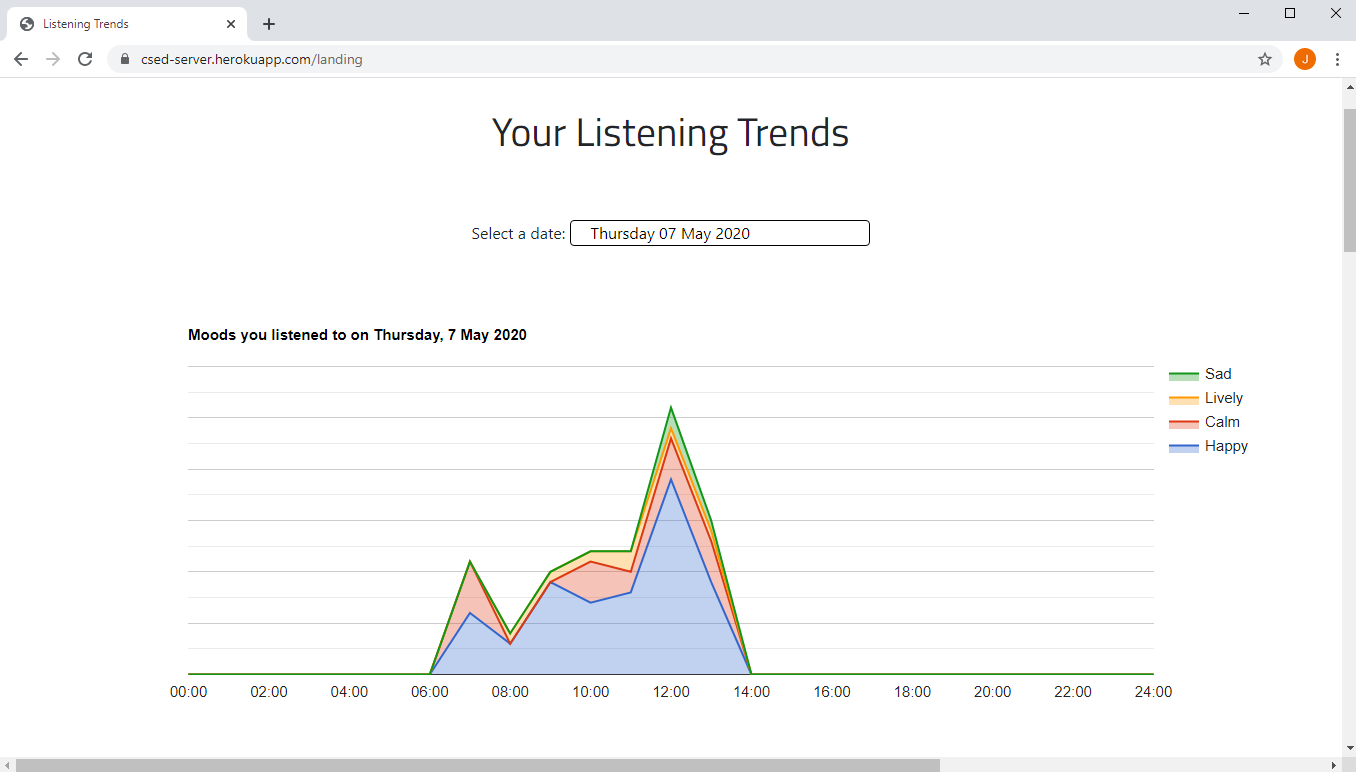
\includegraphics[width=\linewidth]{test/Test37-1.png}
	\caption{Test 37 Part 1}
	\label{fig:test37-1}
\end{subfigure}
\begin{subfigure}{0.4\textwidth}
	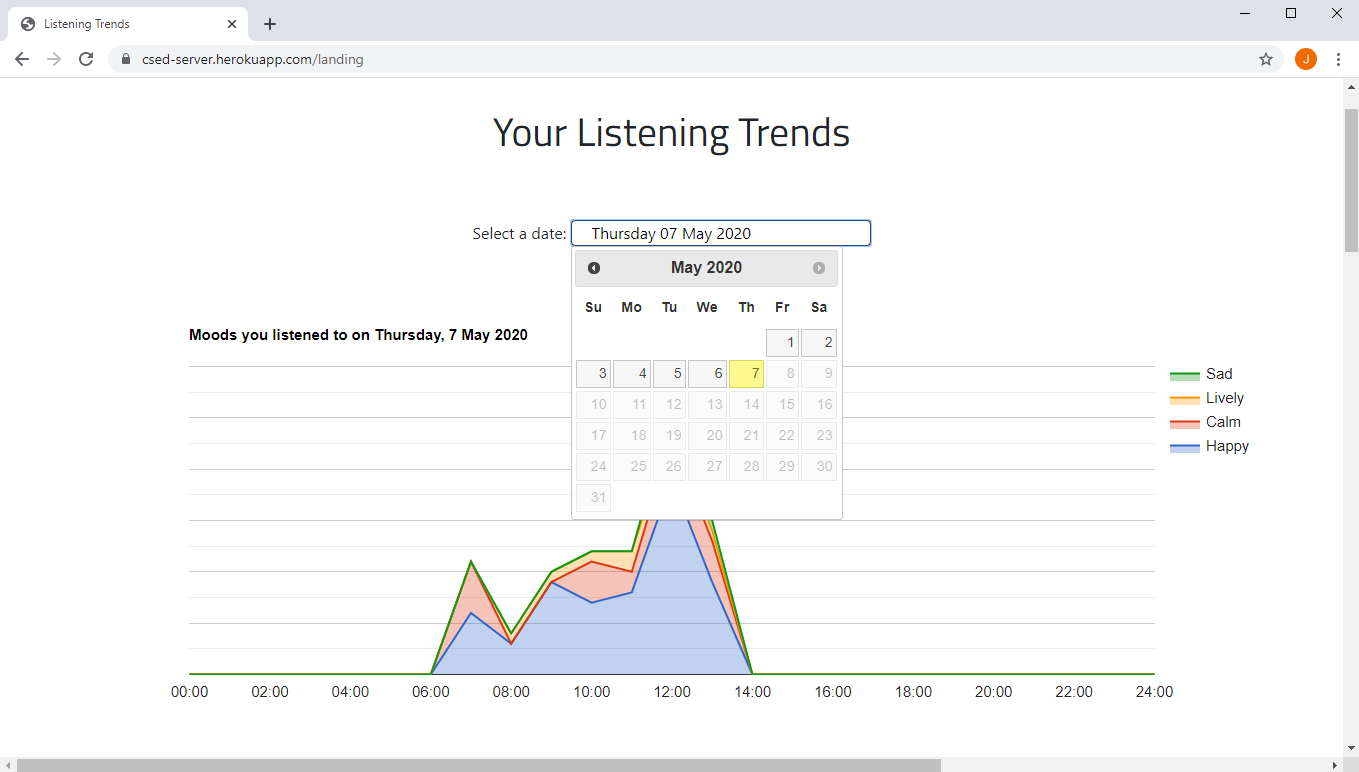
\includegraphics[width=\linewidth]{test/Test37-2.png}
	\caption{Test 37 Part 2}
	\label{fig:test37-2}
\end{subfigure}
\begin{subfigure}{0.4\textwidth}
	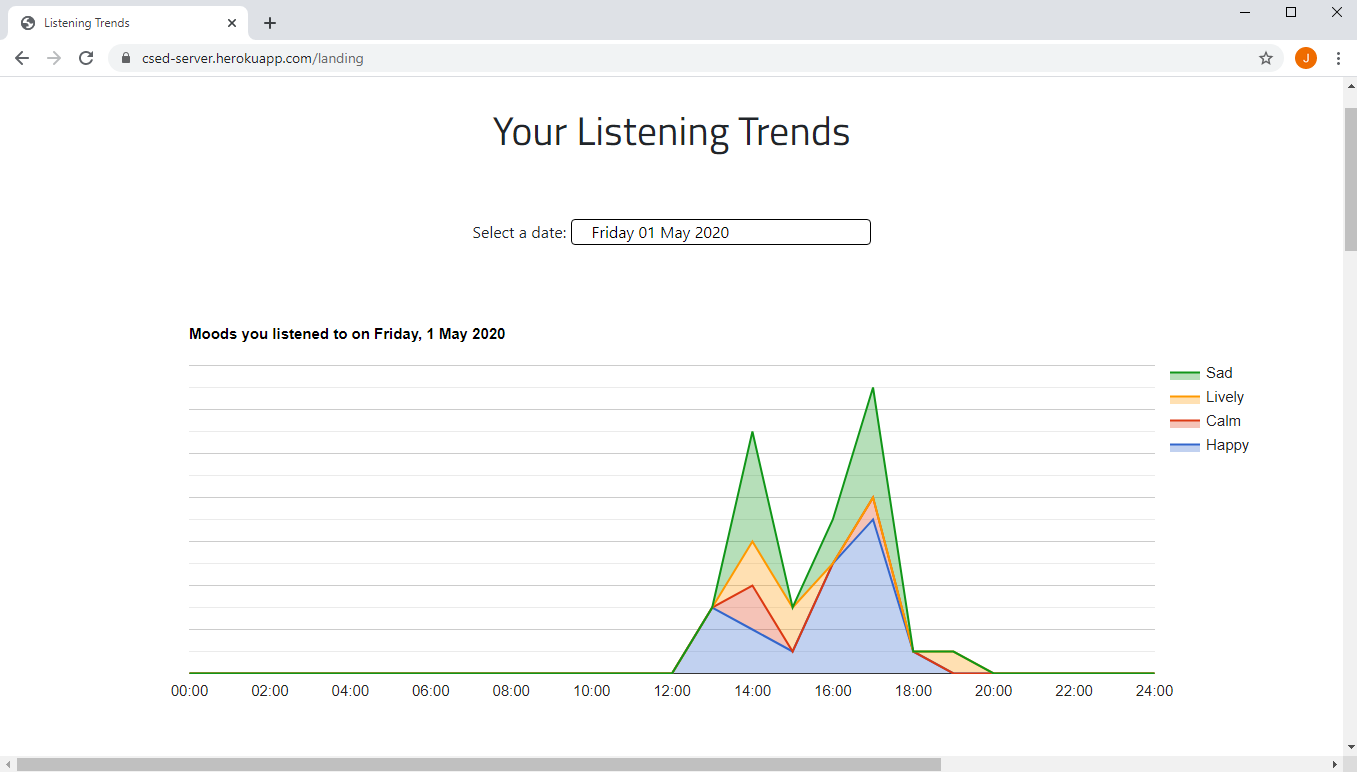
\includegraphics[width=\linewidth]{test/Test37-3.png}
	\caption{Test 37 Part 3}
	\label{fig:test37-3}
\end{subfigure}
\caption{Test 37}
\label{fig:test37}
\end{figure}
\newpage
\testedv{38}
\testedv{39}


\section{Evidence of Agile Approach}
\label{sec:agileapp}

\subsection{Sprint 1}

\begin{figure}[!h]
\centering
\begin{subfigure}{\textwidth}
	\centering	
	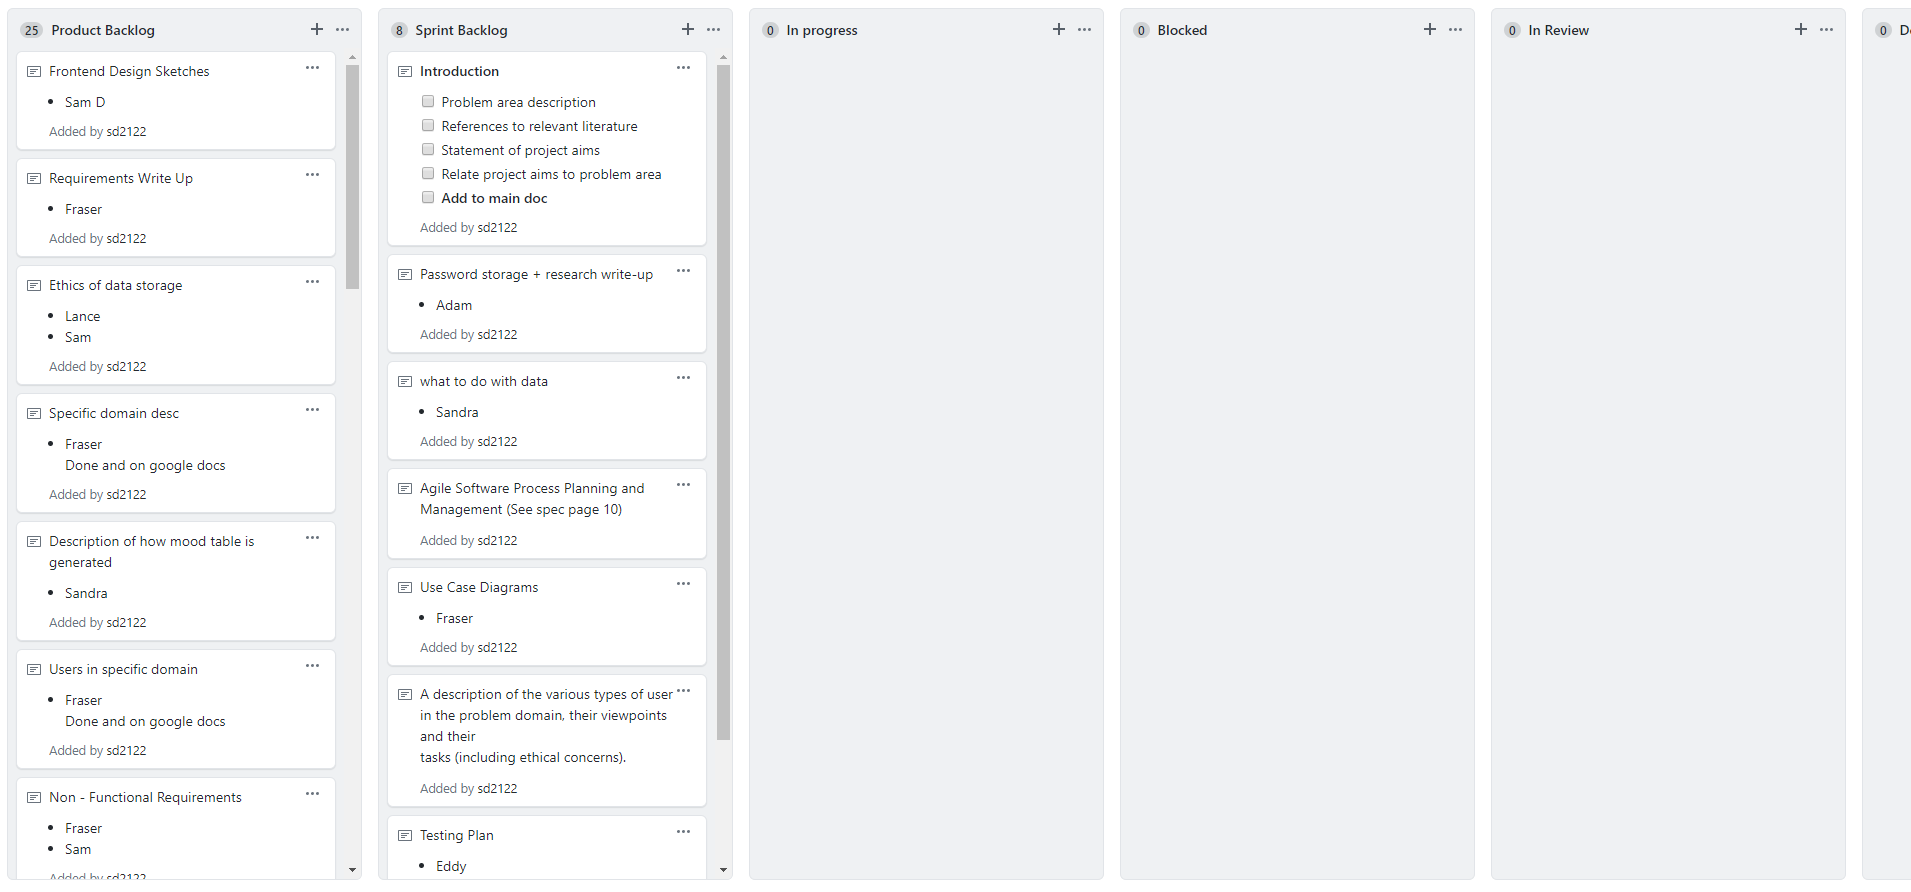
\includegraphics[width=1\linewidth]{git-report-1-before.png}
	\caption{GitHub Report project board before sprint 1}
	\label{fig:agileapp-rb1}
\end{subfigure}
\begin{subfigure}{\textwidth}
	\centering	
	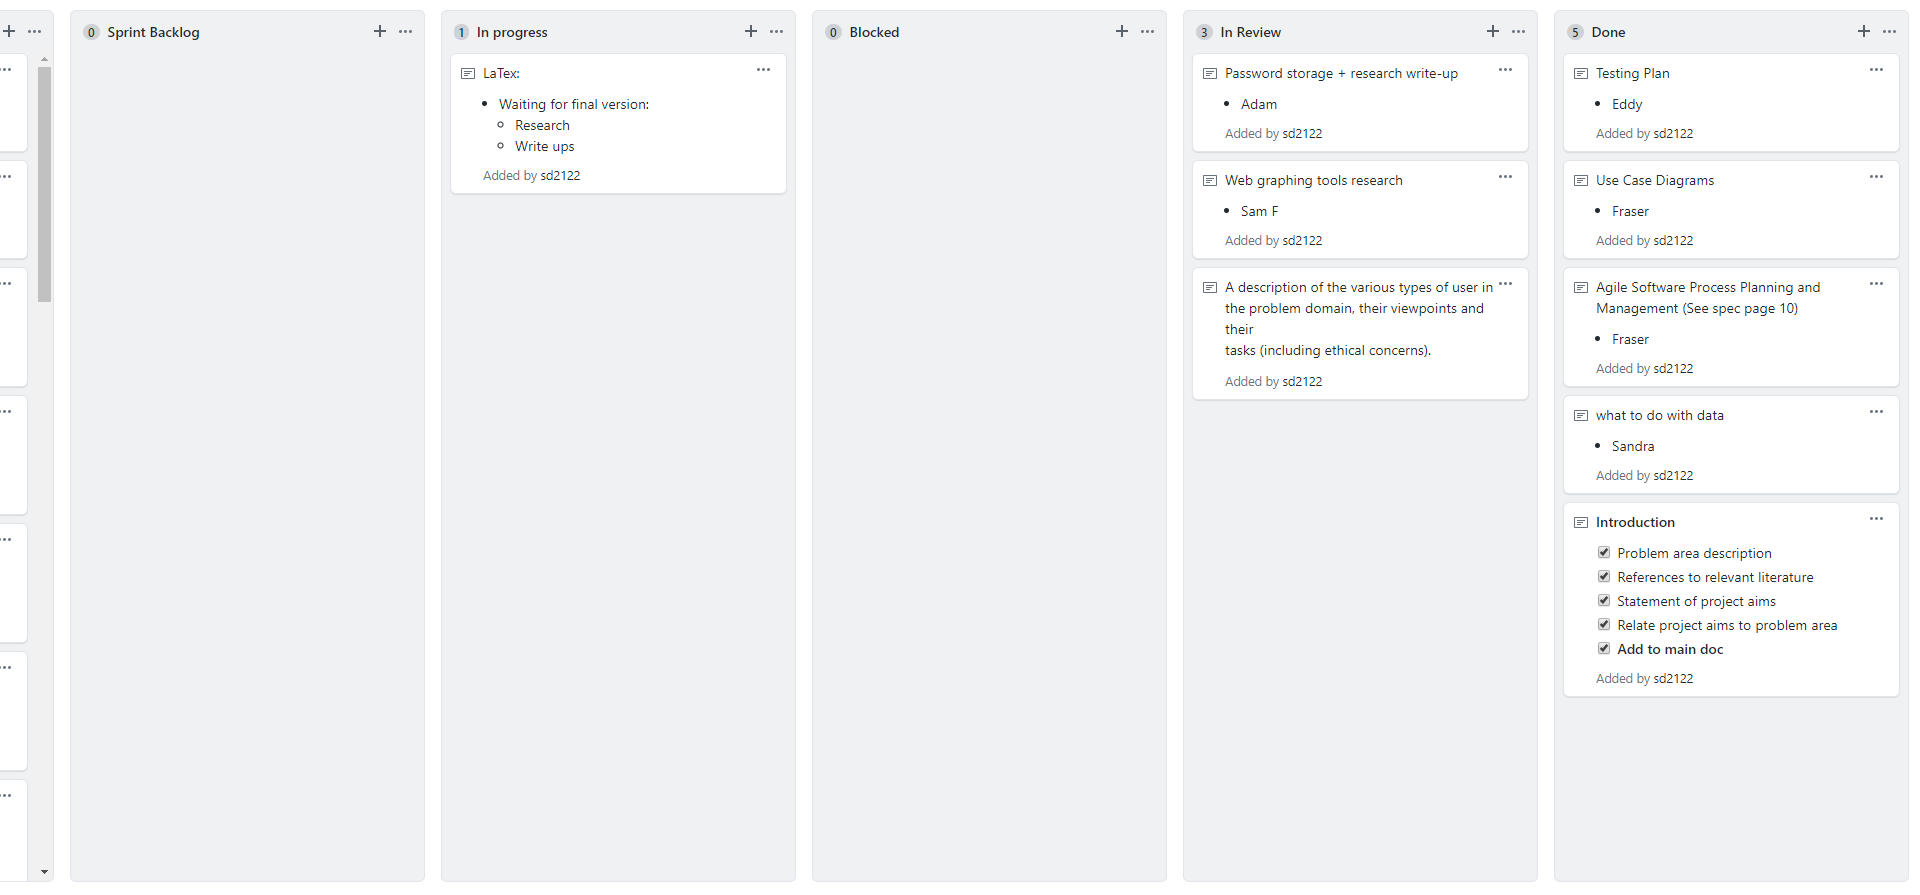
\includegraphics[width=1\linewidth]{git-report-1-after.png}
	\caption{GitHub Report project board after sprint 1}
	\label{fig:agileapp-ra1}
\end{subfigure}

\caption{GitHub report project boards for sprint 1}

\end{figure}

\newpage

\begin{figure}[!h]
\centering
\begin{subfigure}{\textwidth}
	\centering	
	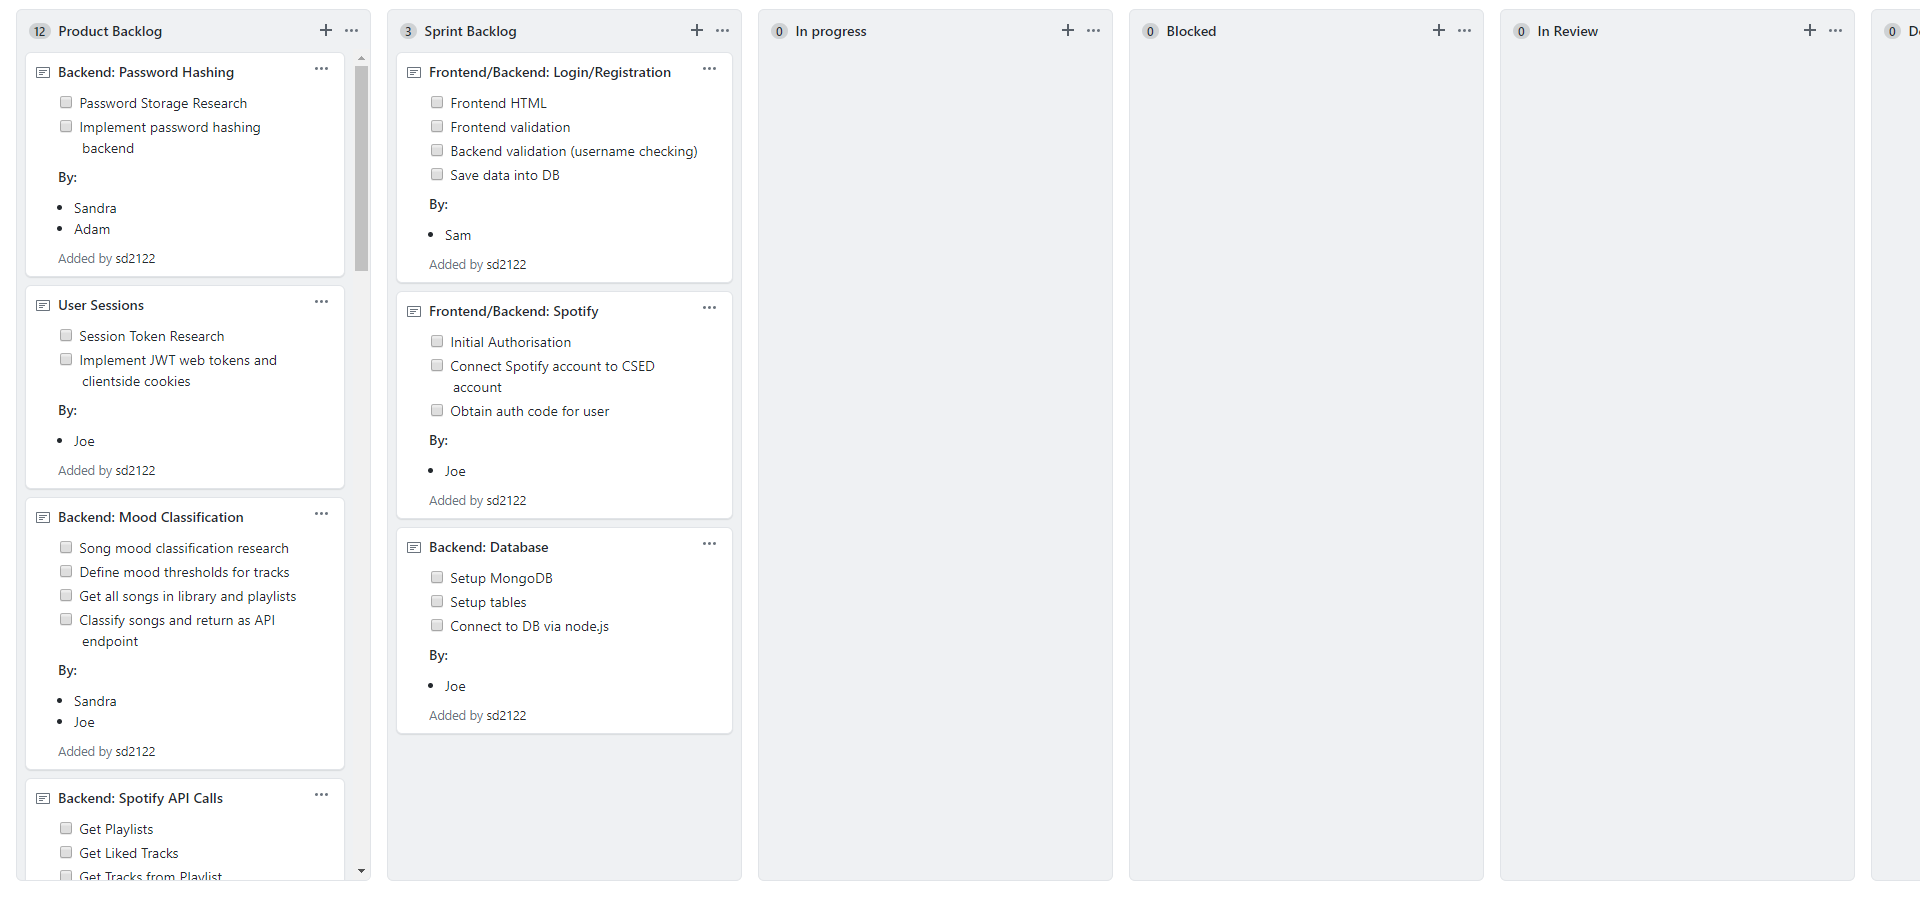
\includegraphics[width=1\linewidth]{git-code-1-before.png}
	\caption{GitHub Code project board before sprint 1}
	\label{fig:agileapp-cb1}
\end{subfigure}
\begin{subfigure}{\textwidth}
	\centering	
	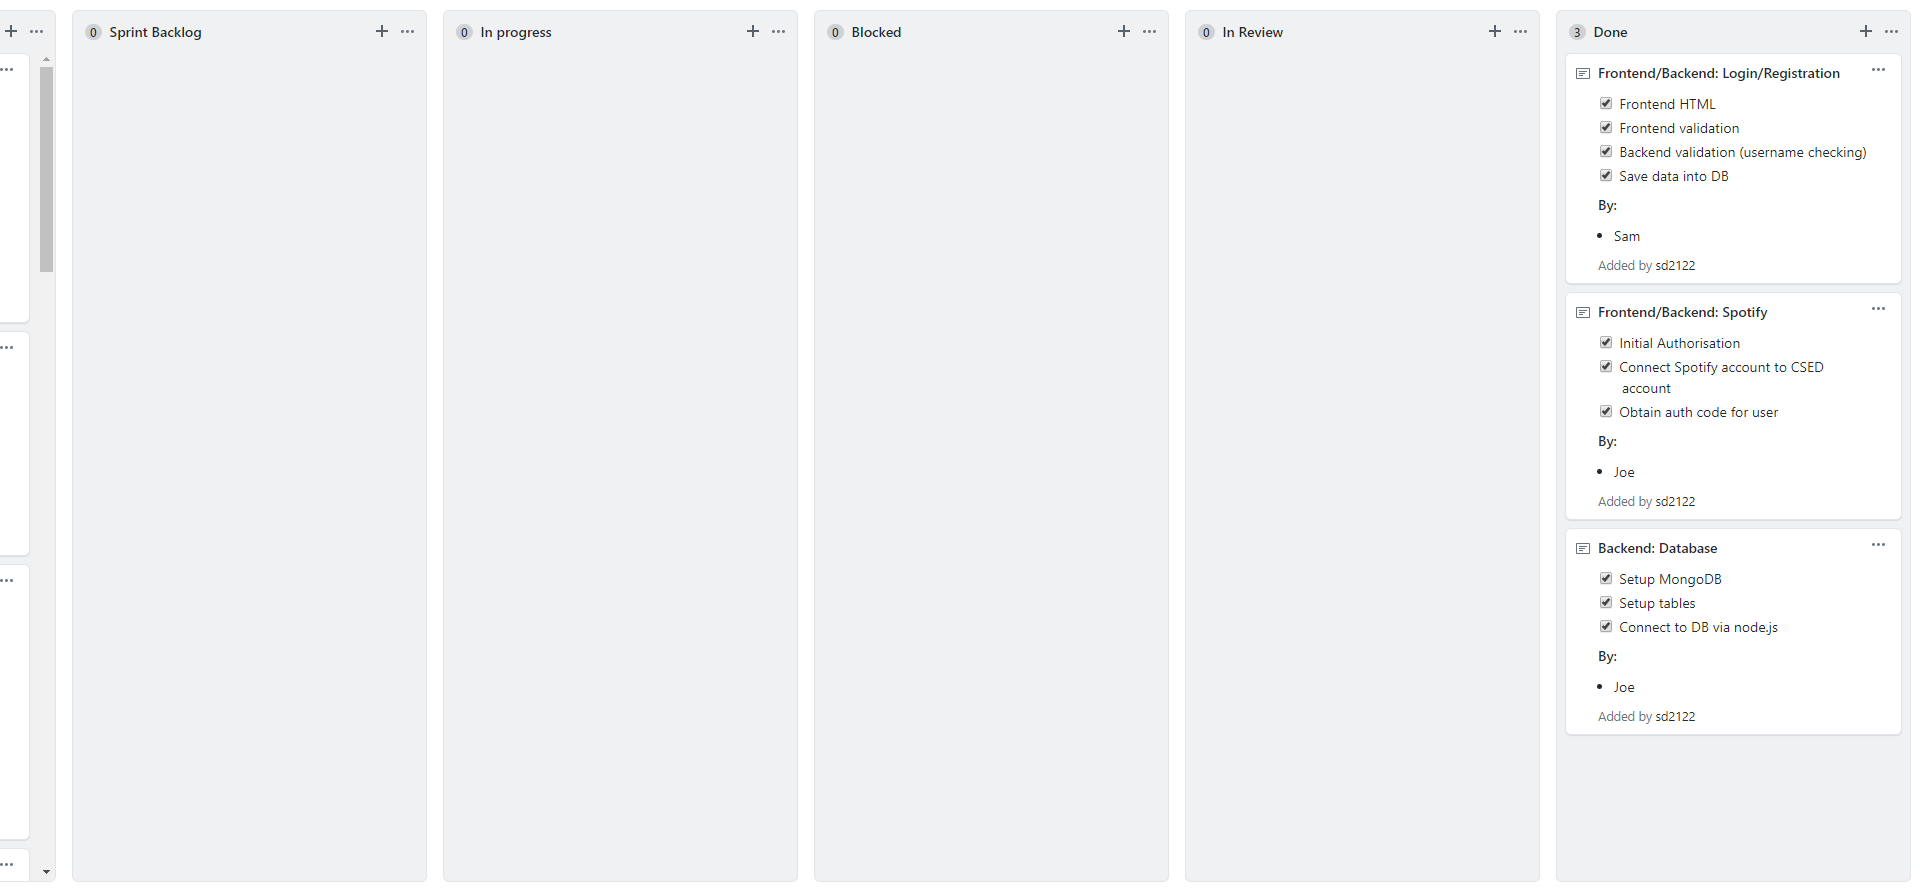
\includegraphics[width=1\linewidth]{git-code-1-after.png}
	\caption{GitHub Code project board after sprint 1}
	\label{fig:agileapp-ca1}
\end{subfigure}

\caption{GitHub code project boards for sprint 1}

\end{figure}

\newpage
\subsection{Sprint 2}

\begin{figure}[!h]
\centering
\begin{subfigure}{\textwidth}
	\centering	
	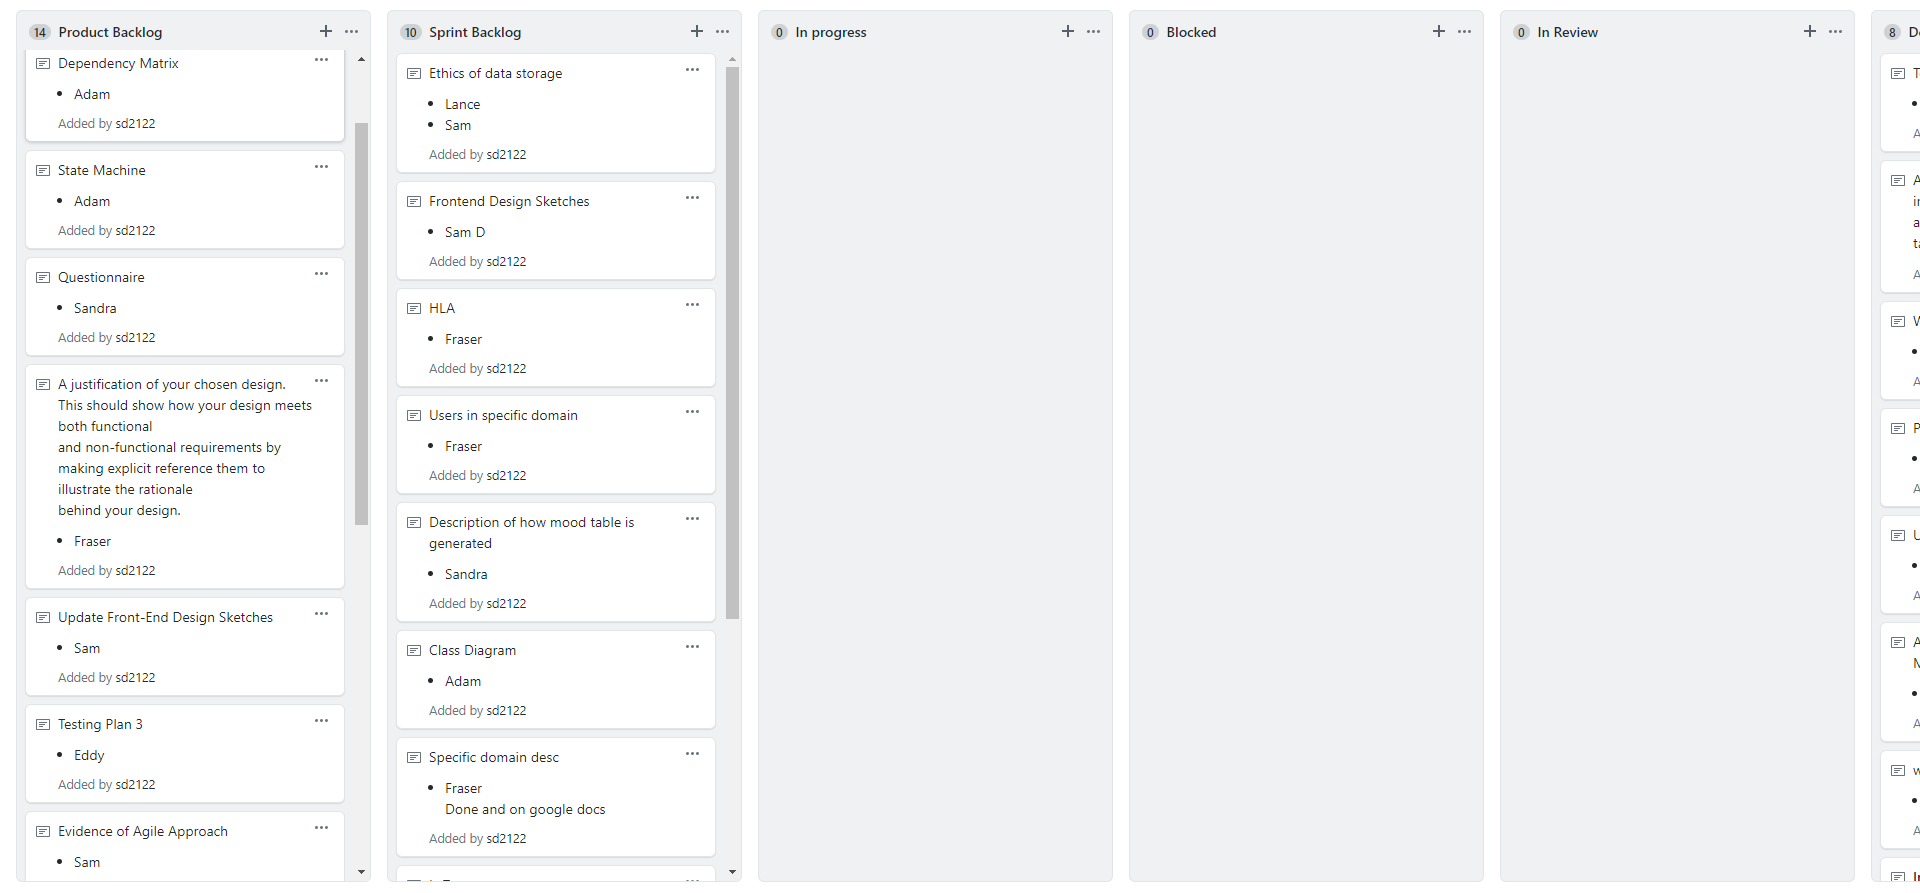
\includegraphics[width=1\linewidth]{git-report-2-before.png}
	\caption{GitHub Report project board before sprint 2}
	\label{fig:agileapp-rb2}
\end{subfigure}
\begin{subfigure}{\textwidth}
	\centering	
	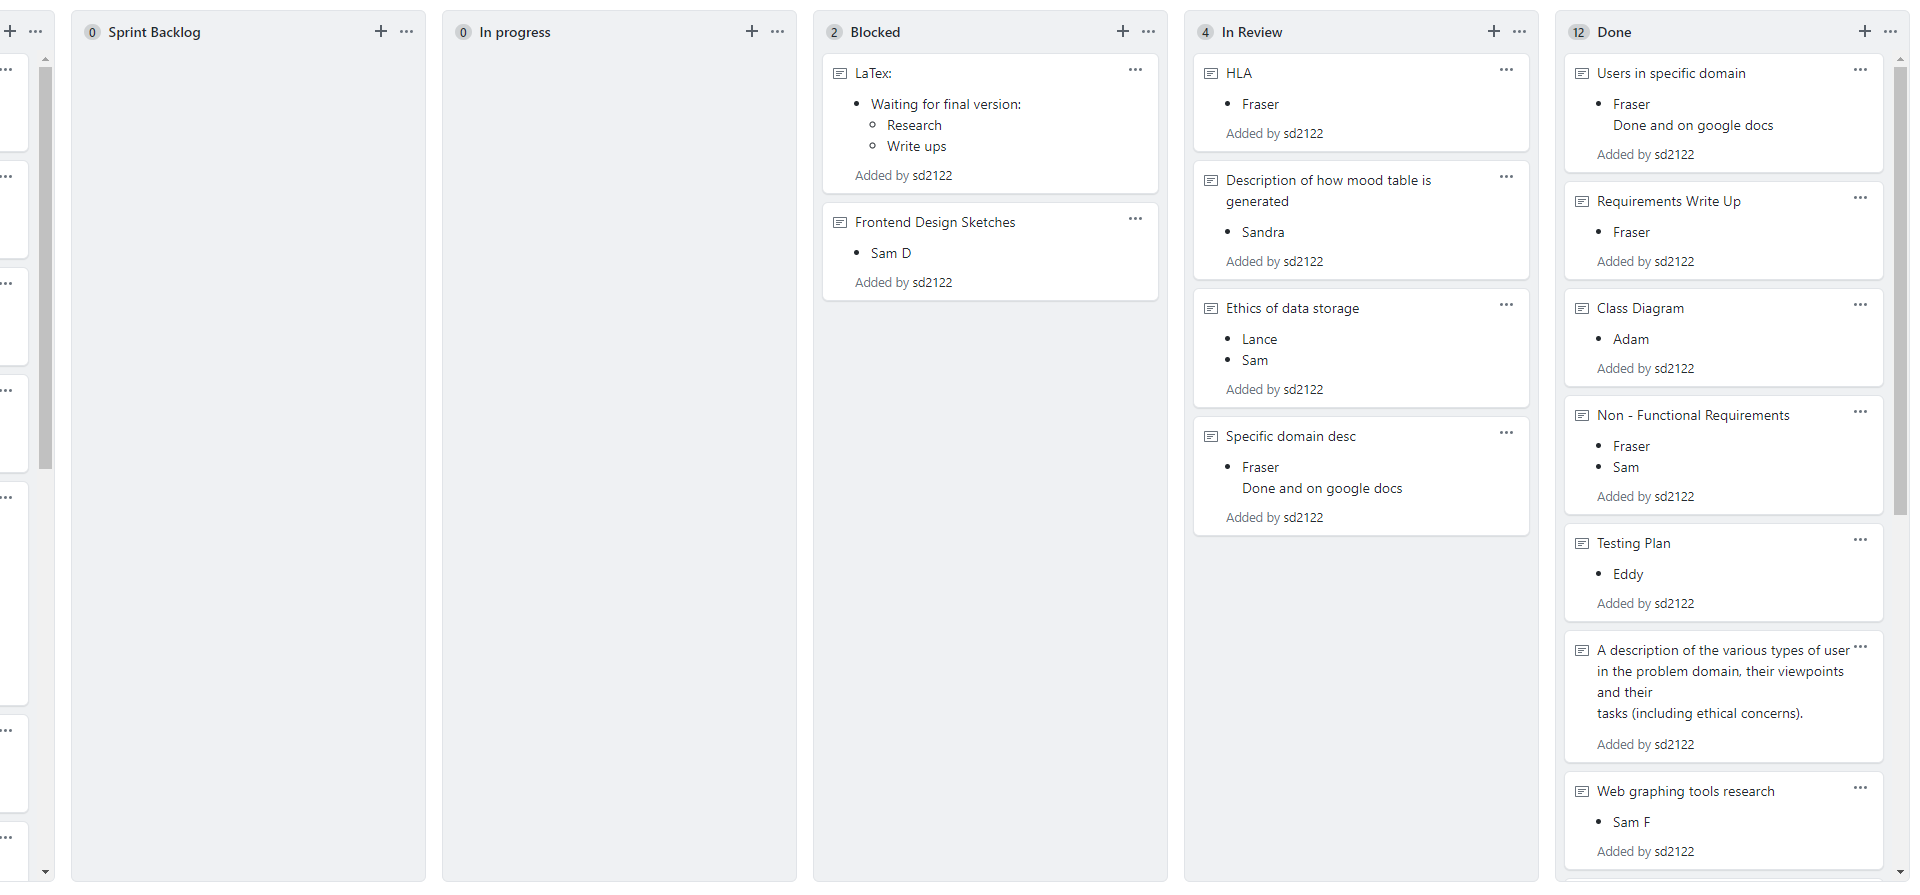
\includegraphics[width=1\linewidth]{git-report-2-after.png}
	\caption{GitHub Report project board after sprint 2}
	\label{fig:agileapp-ra2}
\end{subfigure}

\caption{GitHub report project boards for sprint 2}

\end{figure}

\newpage

\begin{figure}[!h]
\centering
\begin{subfigure}{\textwidth}
	\centering	
	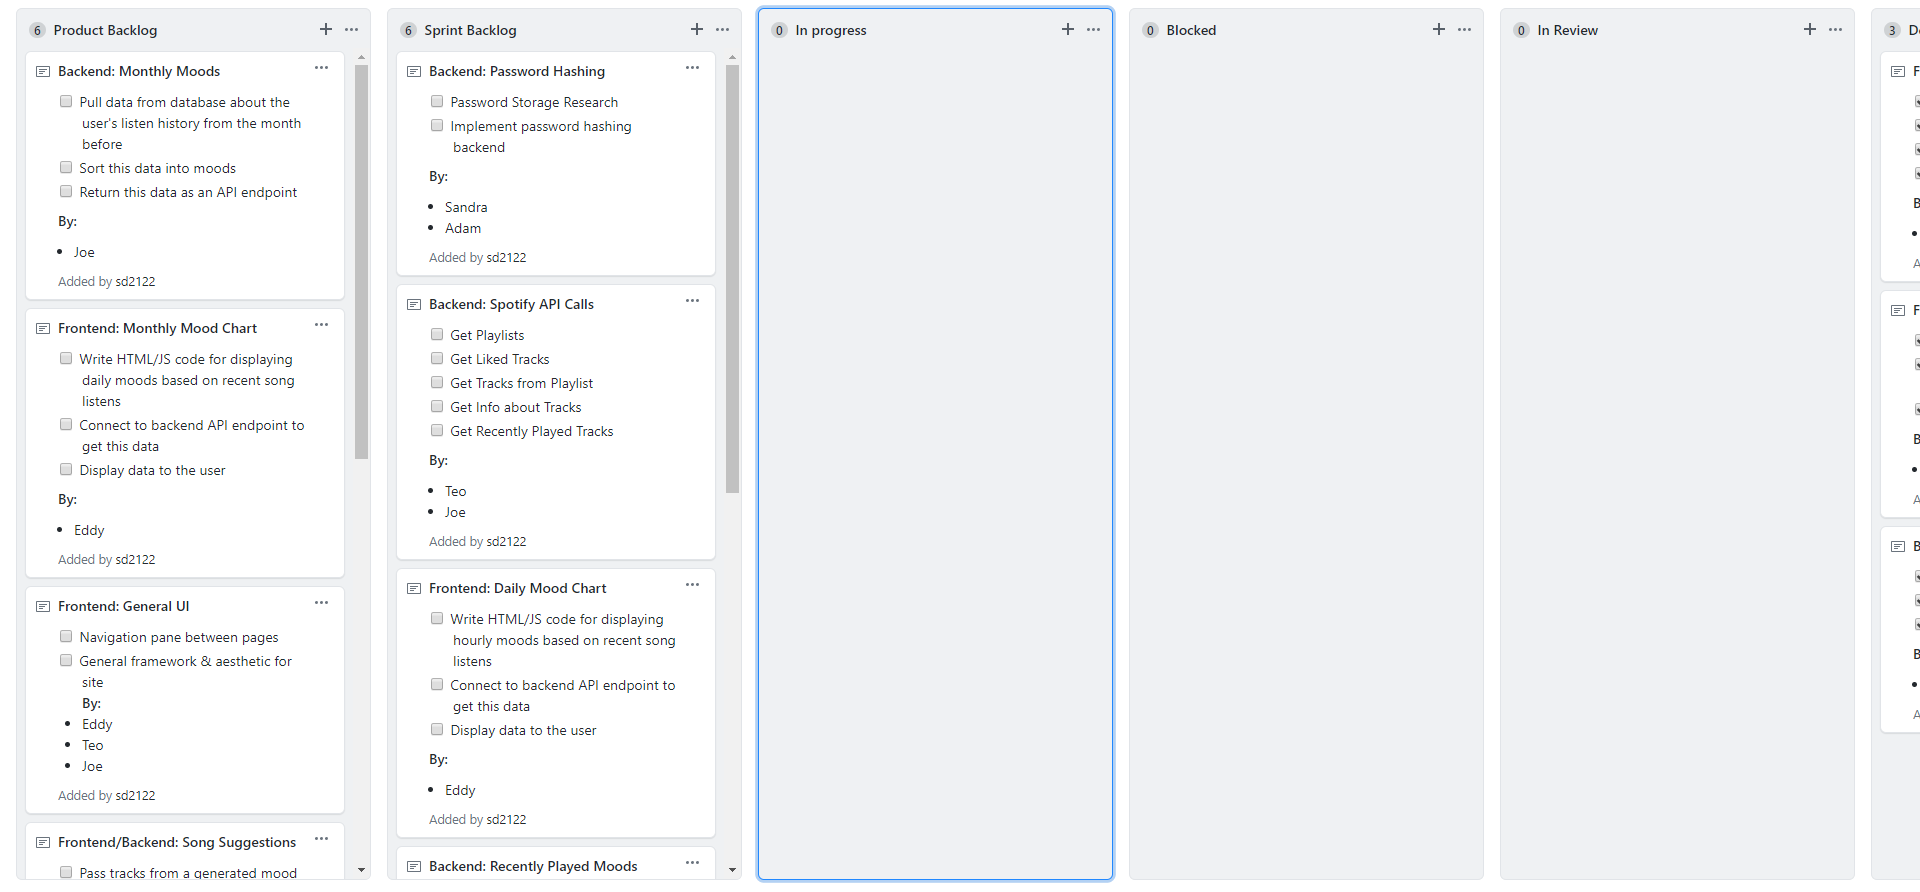
\includegraphics[width=1\linewidth]{git-code-2-before.png}
	\caption{GitHub Code project board before sprint 2}
	\label{fig:agileapp-cb2}
\end{subfigure}
\begin{subfigure}{\textwidth}
	\centering	
	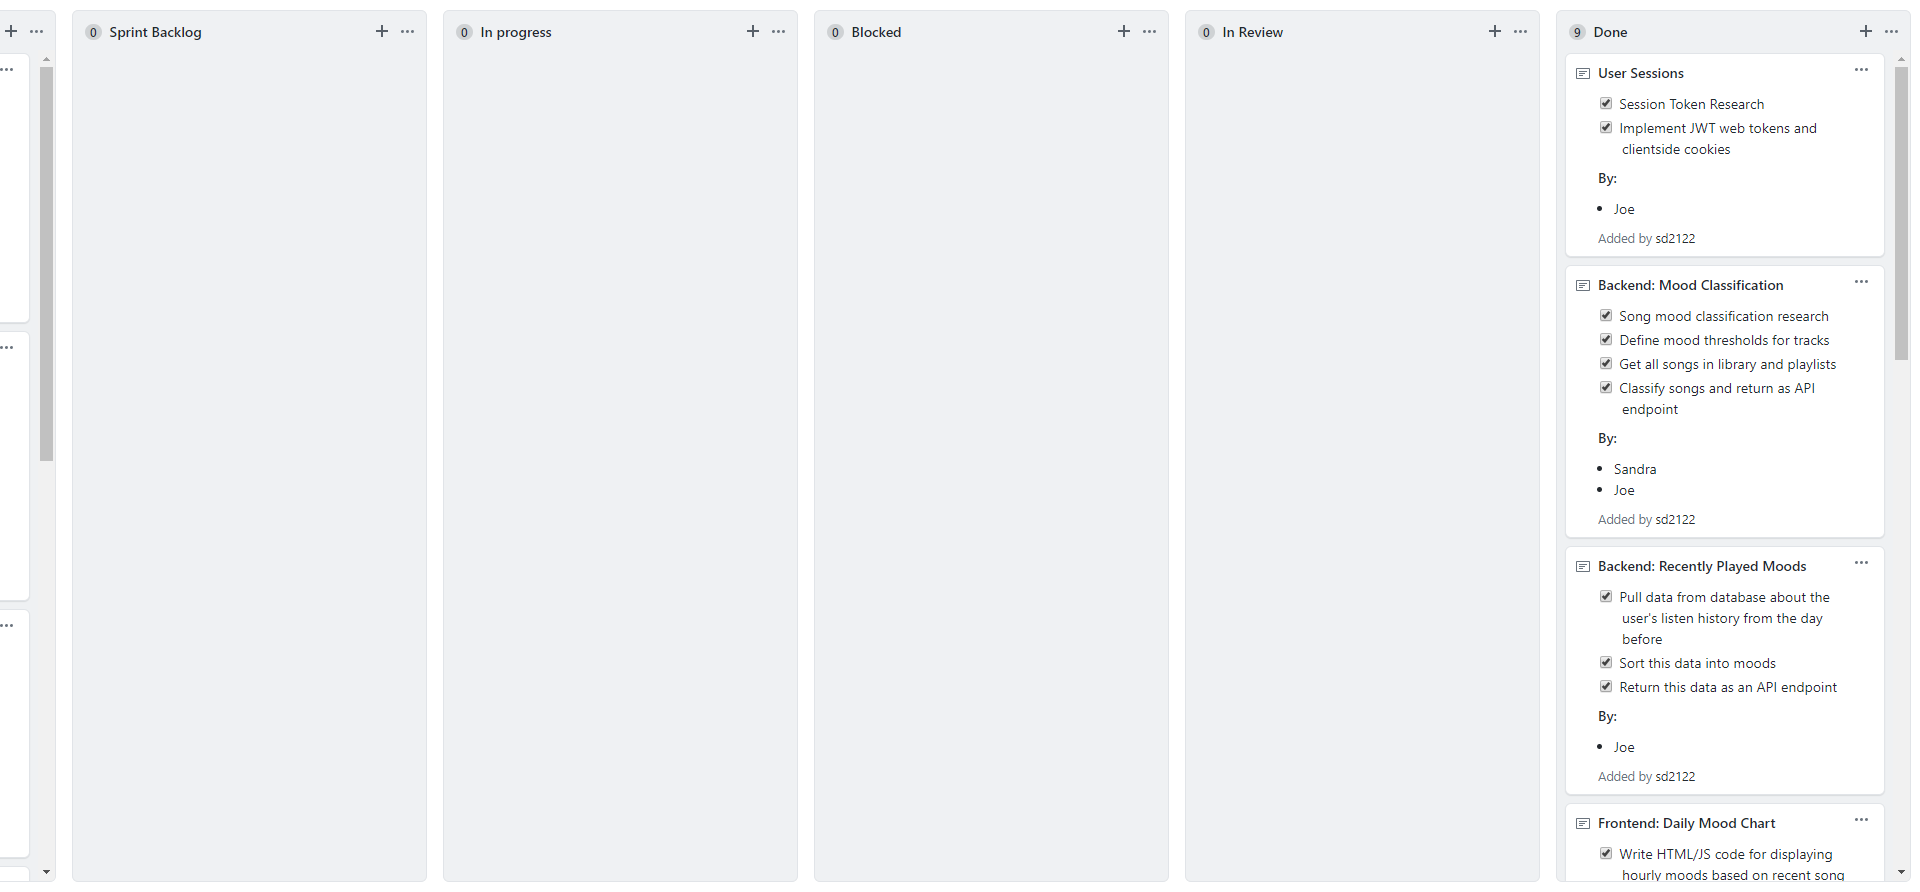
\includegraphics[width=1\linewidth]{git-code-2-after.png}
	\caption{GitHub Code project board after sprint 2}
	\label{fig:agileapp-ca2}
\end{subfigure}

\caption{GitHub code project boards for sprint 2}

\end{figure}
\newpage
\subsection{Sprint 3}

\begin{figure}[!h]
\centering
\begin{subfigure}{\textwidth}
	\centering	
	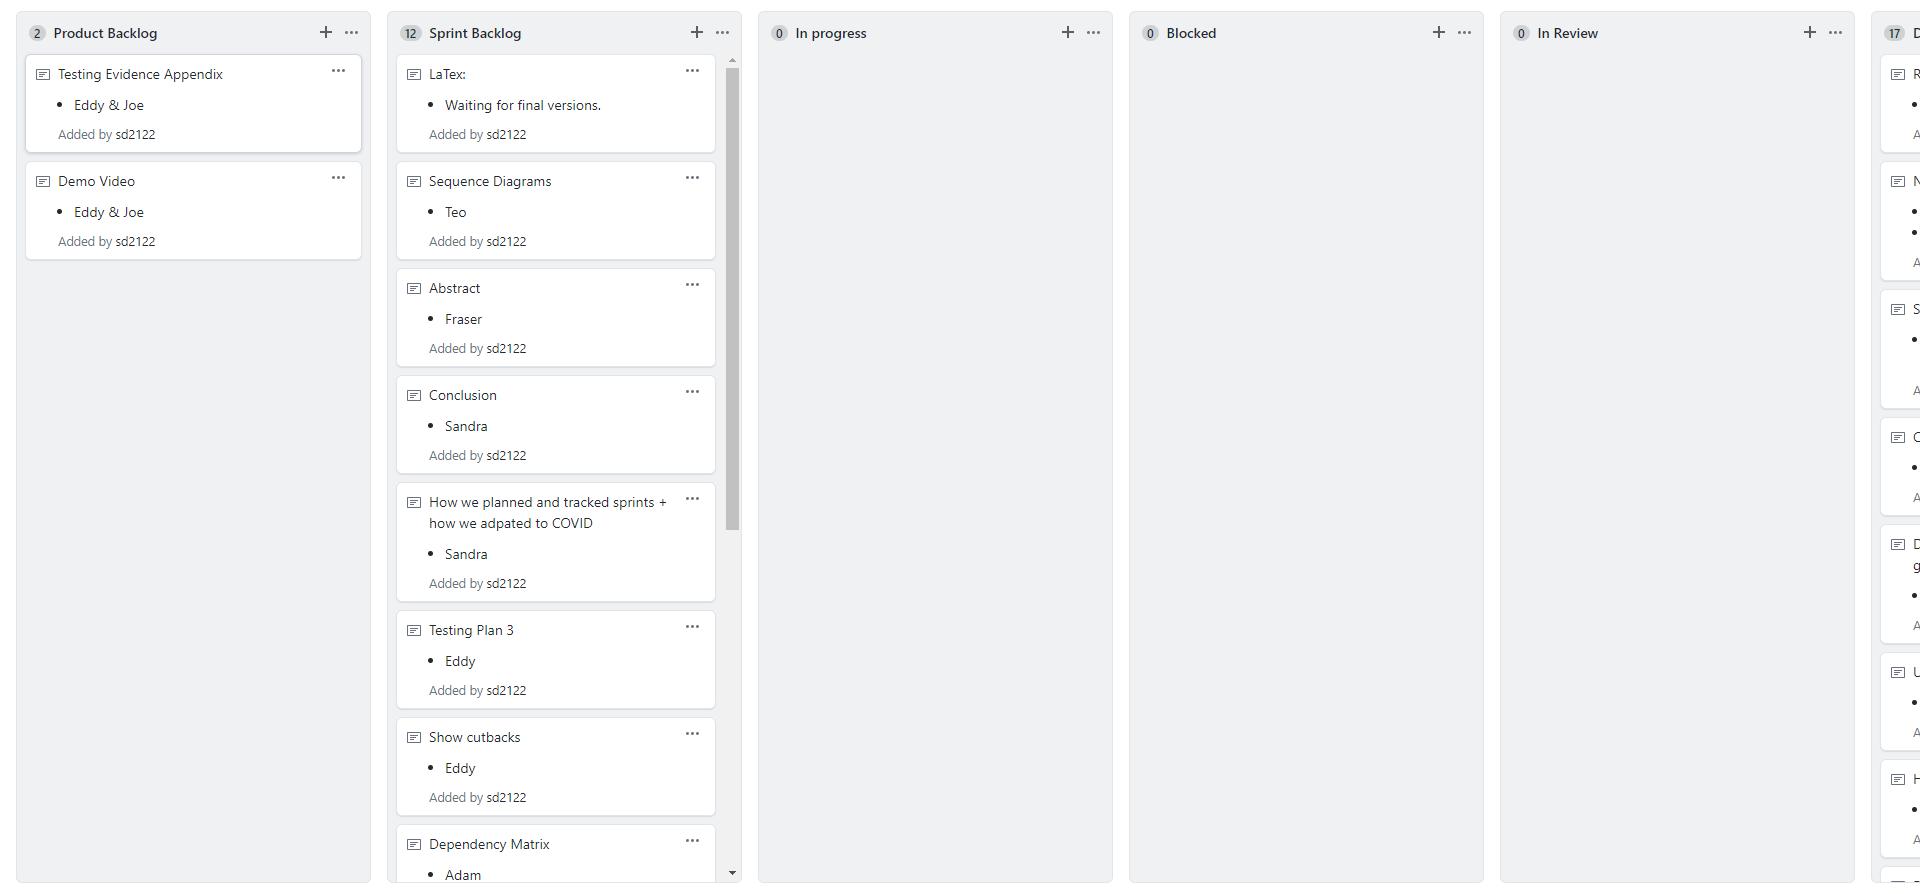
\includegraphics[width=1\linewidth]{git-report-3-before.png}
	\caption{GitHub Report project board before sprint 3}
	\label{fig:agileapp-rb3}
\end{subfigure}
\begin{subfigure}{\textwidth}
	\centering	
	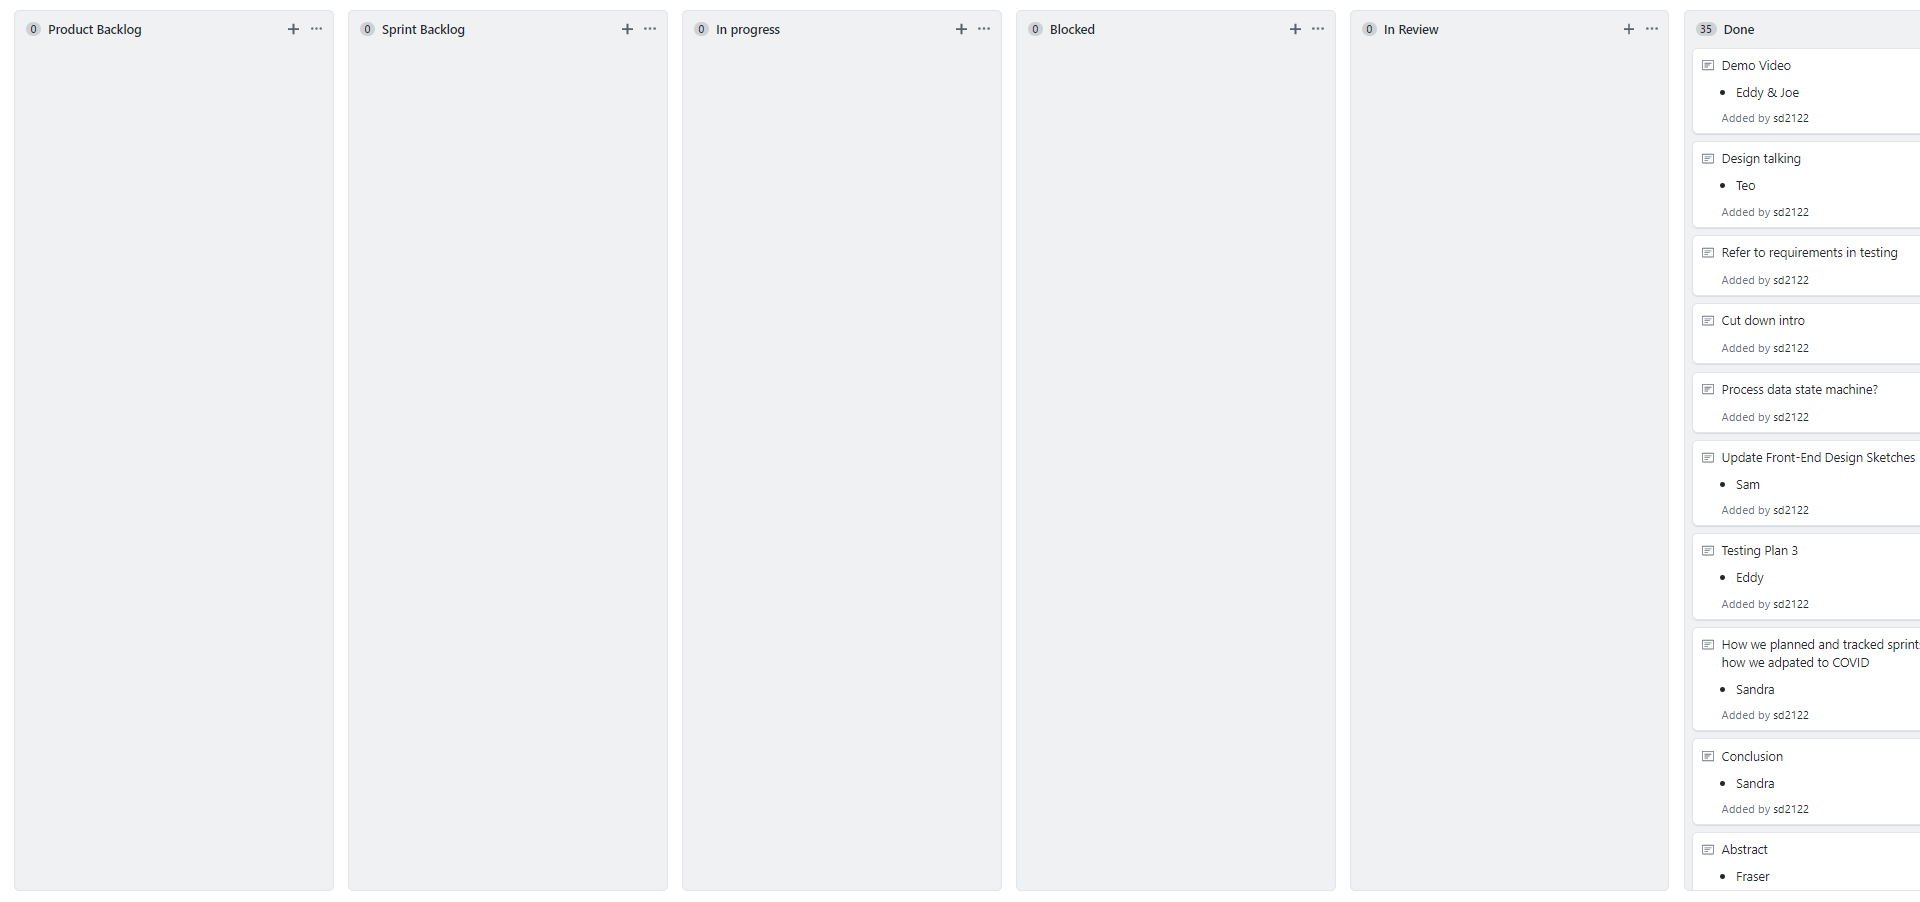
\includegraphics[width=1\linewidth]{git-report-3-after.png}
	\caption{GitHub Report project board after sprint 3}
	\label{fig:agileapp-ra3}
\end{subfigure}

\caption{GitHub report project boards for sprint 3}

\end{figure}

\begin{figure}[!h]
\centering
\begin{subfigure}{\textwidth}
	\centering	
	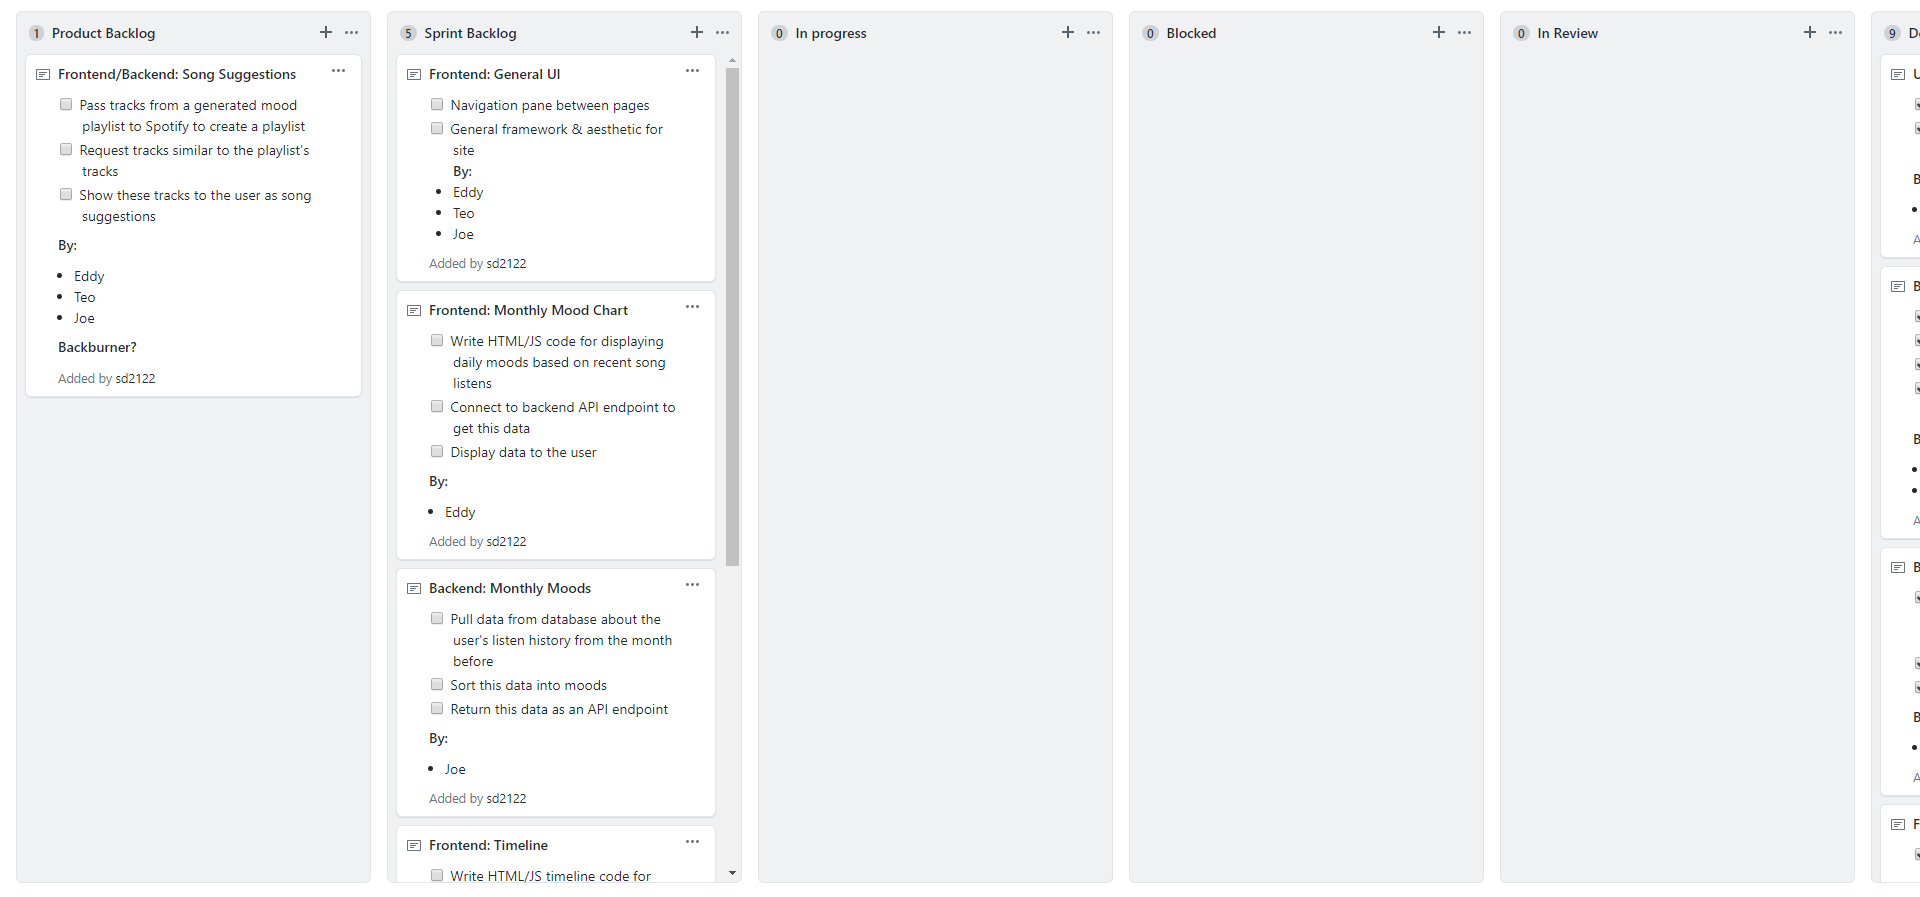
\includegraphics[width=1\linewidth]{git-code-3-before.png}
	\caption{GitHub Code project board before sprint 3}
	\label{fig:agileapp-cb3}
\end{subfigure}
\begin{subfigure}{\textwidth}
	\centering	
	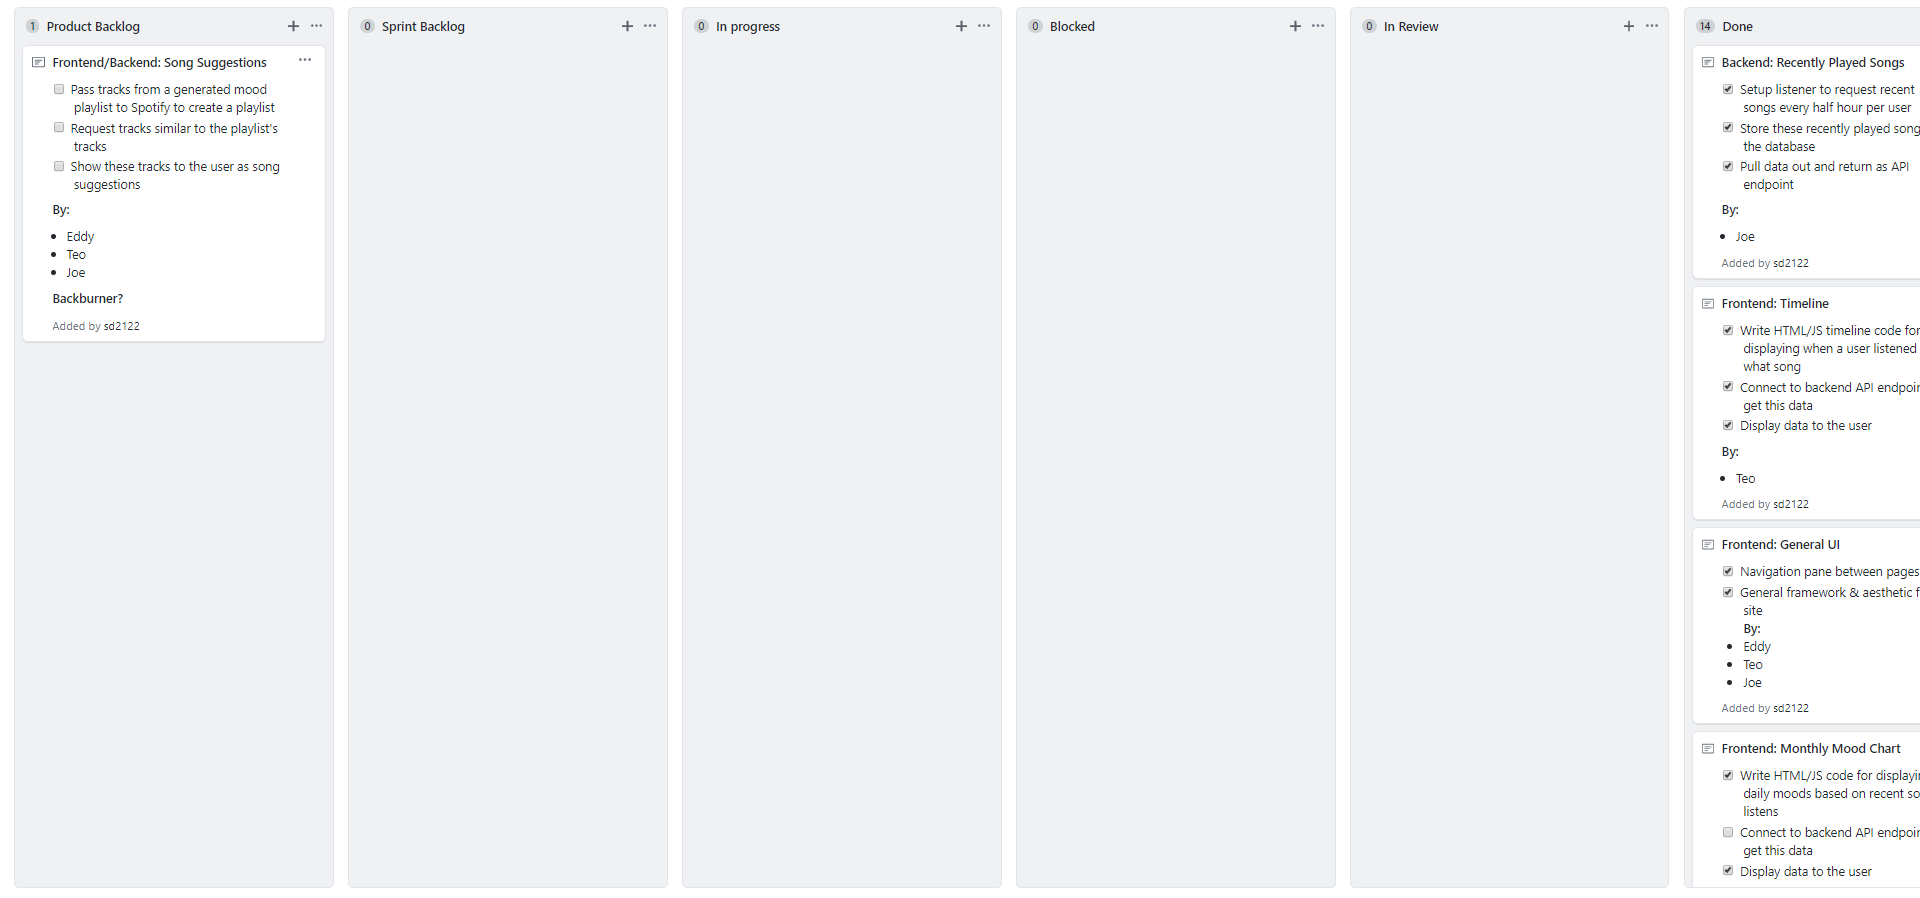
\includegraphics[width=1\linewidth]{git-code-3-after.png}
	\caption{GitHub Code project board after sprint 3}
	\label{fig:agileapp-ca3}
\end{subfigure}

\caption{GitHub code project boards for sprint 3}

\end{figure}
\newpage


\section{Meeting Minutes}

Exact meeting minutes as they were recorded can be found below\\

\subsubsection{13th Feburary 2020}

\begin{lstlisting}
Minutes 13/02/2020

Attendance:
Sandra-maria
Joseph
Sam D
Eddy
Sam F
Lance

- Made a group chat
- Making list of things that could go wrong
- Decided to meet on Mondays 11:15 - 12:00 1 West CS Lab

Goals for next meeting (Monday):
- Get GitHub
- Read through spec
- Actually come to meetings
\end{lstlisting}

\leavevmode \\
\subsubsection{17th Feburary 2020}

\begin{lstlisting}
Minutes 17/02/2020

Attending:
- Teo
- Sam 1 + 2
- Lance
- Eddy
- Sandra
- Adam
- Joe
- Fraser

Minutes:

Key points on spec: 
	code quality not important
	data can be fake

Ideas for project:
	Dietting tracking
	Music tracking

Decided on music tracking

Personal projects dealt out:

Fraser:
A description of the problem area (Personal Informatics) supported by references to goodquality contemporary literature.

Sam D:
A clear statement of the main aim of your software system as a potential solution in theproblem area.

Others:
Gather articles for research and a short paragraph on what they're about
\end{lstlisting}

\leavevmode \\
\subsubsection{20th of Feburary 2020}

\begin{lstlisting}
Minutes 20/02/2020
Attendance:
- Sam F
- Sam D
- Eddy
- Lance
- Sandra
- Adam
- Fraser
- Teo
- Joe

Minutes: 12.15pm - 13.05pm
Key Points
-	Music Tracking, looking into a different users patterns.
-	Mood assumptions based on the type of music they are listening to.
-	Is the project ethical.
Joe, Teo, Lance:
-	Requirements.
Sandra:
-	Ethics
Eddy, Sam F, Adam:
-	Research, data collection and representation
Eddy:
-	Latex 

By next meeting:
-	Introduction
-	Started requirements.
-	Begin looking into ethics.
-	Additional research.
\end{lstlisting}

\leavevmode \\
\subsubsection{24th of Feburary 2020}

\begin{lstlisting}
Minutes 24/02/2020
Attendance:
- Eddy
- Teo
- Sam D
- Sandra
- Adam
- Sam F
Minutes: 11.15am - 12pm
Key Points
-	Continue requirements and ethics.

By next meeting:
-	Finish requirements.
-	Begin our first sprint.
\end{lstlisting}

\leavevmode \\
\subsubsection{27th of Feburary 2020}

\begin{lstlisting}
Minutes 27/02/2020
Attendance:
- Sam F
- Sam D
- Eddy
- Sandra
- Adam
- Fraser
- Joe

Minutes: 12:15pm - 1:05pm

Potential Features list:
- Serverside listener 
	- Listen = 30 seconds+
	- Database
		- Make an object class
		- Setup tables
	- Connect to Spotify Web API
	- Setup Web API for client
- Client
	- UI
	- Receive from server Web API	
	- Good visualisation of data
		- Timeline of your listening history
		- Recommendations
\end{lstlisting}

\leavevmode \\
\subsubsection{2nd of March 2020}

\begin{lstlisting}
02/03/20

In Attendance
-Eddy
-Fraser
-Joe
-Sam
-Sandra
-Adam
-Lance
-Teo

TODO:
-Research password security
-Ethics of security
-Write sprint into GitHub
-Add report requirements to GitHub

Decided:
-Languages: Front: JS, HTML, CSS; Back: Node and SQLite
\end{lstlisting}

\leavevmode \\
\subsubsection{5th of March 2020}

\begin{lstlisting}
Minutes 05/03/2020
Attendance:
- Joe
- Fraser
- Sandra
- Adam
- Teo
- Eddy
- Sam D

Key points:
- Add a test plan for end of sprint.
- Sprint is going to plan.
- Everyone continue their sprint jobs.

Eddy:
- Test plan for sprint.

Eddy, Fraser:
- Work on UML Diagrams.
\end{lstlisting}

\leavevmode \\
\subsubsection{10th of March 2020}

\begin{lstlisting}
Minutes 10/03/2020
Attendance:
- Adam
- Joe
- Sandra
- Fraser
- Sam D

Main points:

- Catch up on where everyone is.
- Allocated new jobs to people.
- Checked for issues on the jobs in progress.

For next meeting:

- Finish jobs.
- Put all work together, presented nicely.
\end{lstlisting}

\leavevmode \\
\subsubsection{13th of March 2020 at 12:00}

\begin{lstlisting}
Meeting Minutes 12:00 12/3/20

Attendance:
- Joe
- Sam F
- Fraser
- Sandra
- Lance

What was Discussed:
- Where we had all got up to with our previous tasks
- What is still left to do before our sprint review

Before next meeting:
- Finish risk assessment before sprint review
- Split up more tasks
\end{lstlisting}

\leavevmode \\
\subsubsection{13th of March 2020 at 17:00}

\begin{lstlisting}
Meeting Minutes 17:00 12/3/20

Attendence:
- Joe
- Fraser 
- Sandra
- Adam
- Sam F

What was done:
- More hashing research 
- Hashing was implemented
- Test plan was altered
- Sprint review carried out
- Added more tasks to product backlog in preparation for second sprint

Before next meeting:
- Choose your own task from the product backlog and try complete before next sprint
- Next sprint starting monday 16-3-20
\end{lstlisting}

\leavevmode \\
\subsubsection{16th of March 2020}

\begin{lstlisting}
Meeting Minutes 16-03-20

Attendance:
- Fraser
- Eddy
- Sam F
- Teo
- Sam D

What was done:
- Talked about what had been done since sprint review
- Sorted out what needed to be done for sprint 2
- Split up work
- Planned to start sprint 19-03-20

Before next meeting:
- Finish all work that needs to be done before next sprint
- Sort out alternate comminication method due to Covid-19
	- Microsoft Teams
\end{lstlisting}

\leavevmode \\
\subsubsection{19th of March 2020}

\begin{lstlisting}
Meeting Minutes 19-03-20

Attendance:
- Sam D
- Fraser
- Sandra
- Adam

What was done: 
- Discussed what had been done since last meeting
- Tried to get everyone on our first Microsoft Teams meeting
- Talked about where we were with the project
	- What needs to be done by next meeting
	- Rough time frame for the rest of the project

Before Next meeting:
- Carry on with work from last meeting
	- Improve something that you had finished
\end{lstlisting}

\leavevmode \\
\subsubsection{23rd of March 2020}

\begin{lstlisting}
Minutes 23/03/2020
Attendance:
- Fraser
- Sam F
- Sandra
- Sam D

Key points:
- See where everyone is. 
- Discussed the types of requirements we will need for the system.
- Completed introduction.

- Get in contact with the others and see if they are settled.
\end{lstlisting}

\leavevmode \\
\subsubsection{26th of March 2020}

\begin{lstlisting}
Minutes 26/03/2020
Attendance:
- Adam
- Joe
- Eddy
- Sam F
- Sam D
- Fraser
- Sandra

Key points:
- Created a document which we will throw all final versions of write ups to add to the LaTex document.
- Discussed where we are currently and we had to do before the end of the sprint.
\end{lstlisting}

\leavevmode \\
\subsubsection{30th of March 2020}

\begin{lstlisting}
Minutes 30/03/2020
Attendance:
- Sam D
- Eddy
- Sandra
- Fraser

Key points:
- Quick meeting as not everyone was there.
- Seen if people in the meeting were on track and had something to do.

- Meeting with the whole group next time.
\end{lstlisting}

\leavevmode \\
\subsubsection{2nd of April 2020}

\begin{lstlisting}
Minutes 02/04/2020
Attendance:
- Teo
- Sandra
- Eddy
- Joe
- Sam D
- Adam

Key points:
- Reviewed what we did in sprint 1.
- Plan what must be done in sprint 2.
- Make minor adjustments to current documentation.

- Ethics
- Design
- Continue research on moods for the code.
\end{lstlisting}

\leavevmode \\
\subsubsection{9th of April 2020}

\begin{lstlisting}
Minutes 09/04/2020
Attendance:
- Adam
- Sam D
- Joe
- Eddy
- Sandra

Key points:
- Making progress.
- Checking in to see where everyone is.
- Assigned more tasks to those who have finished current ones.

\end{lstlisting}

\leavevmode \\
\subsubsection{14th of April 2020}

\begin{lstlisting}
Minutes 14/04/2020
Attendance:
- Adam
- Eddy
- Fraser
- Sam D
- Sandra
- Joe

Key points:
- Tested the current code, see if it would work with multiple accounts.
- Checked in on everyones progress, continue current jobs.
- Code is somewhat accurate in gathering the mood of a song.
\end{lstlisting}

\leavevmode \\
\subsubsection{16th of April 2020}

\begin{lstlisting}
Minutes 16/04/2020
Attendance:
- Adam
- Joe
- Sam D
- Eddy
- Teo
- Sandra

Key points:
- Discussed where we could improve.
- Discussed what was to be done in the 3rd sprint.
- Everyone must have something to do as this is the last sprint.

- Abstract
- Conclusion
- Minor details we have to change in the documentation.
- Finish code.
\end{lstlisting}

\leavevmode \\
\subsubsection{21st of  April 2020}

\begin{lstlisting}
Minutes 21/04/2020
Attendance:
- Adam
- Eddy
- Sandra
- Teo
- Fraser
- Sam D
- Joe

Key points:
- Retested the code for new features like daily tracking.
- Checked in to see where everyone currently is.
- Made minor changes to the documentation.
- Continue devloping the code.
\end{lstlisting}

\leavevmode \\
\subsubsection{23rd of April 2020}

\begin{lstlisting}
Minutes 23/04/2020
Attendance:
- Sandra
- Joe
- Sam D
- Adam
- Eddy

Key points:
- Pushed for certain things to get done.
- Nearing the end of the sprint so we laid out exactly what had to be done.
\end{lstlisting}

\leavevmode \\
\subsubsection{28th of April 2020}

\begin{lstlisting}
Minutes 28/04/2020
Attendance:
- Sandra
- Joe
- Adam
- Eddy
- Teo
- Fraser

Key points:
- Small meeting to check in on the progress.
- Might need to extend the sprint to make time for minor details of the document and the code.
- Continue doing current tasks.
\end{lstlisting}

\leavevmode \\
\subsubsection{30th of April 2020}

\begin{lstlisting}
Minutes 30/04/2020
Attendance:
- Eddy
- Adam
- Sandra
- Sam D
- Teo

Key points:
- Assign everything that there is left to do to people.
- Finish by Tuesday 5th May.
- Documentation sprint cycle has been updated to show everyone what they have to do.
\end{lstlisting}

\end{document}